\chapter{慢性咳嗽}

咳嗽是一种保护性反射动作,能将呼吸道内分泌物或异物排出体外;另一方面也为病理性,作为呼吸系统疾病的常见症状。当耳、鼻、咽、喉、支气管、胸膜、肺等脏器,由于炎症、淤血、物理、化学或过敏等因素刺激时,通过分布于此等器官的迷走神经分支传达到延髓咳嗽中枢,引起咳嗽反射。目前已把咳嗽分成急性、亚急性和慢性咳嗽(chronic
cough),急性咳嗽定义为咳嗽持续3周以内,亚急性咳嗽为3~8周,慢性咳嗽为8周以上。能引起慢性咳嗽的疾病很多(参考表\ref{tab5-1})。诊断时须注意下列检查:

\section{(一)病史、症状、体征}

\begin{table}[htbp]
\centering
\caption{慢性咳嗽疾病的分类}
\label{tab5-1}
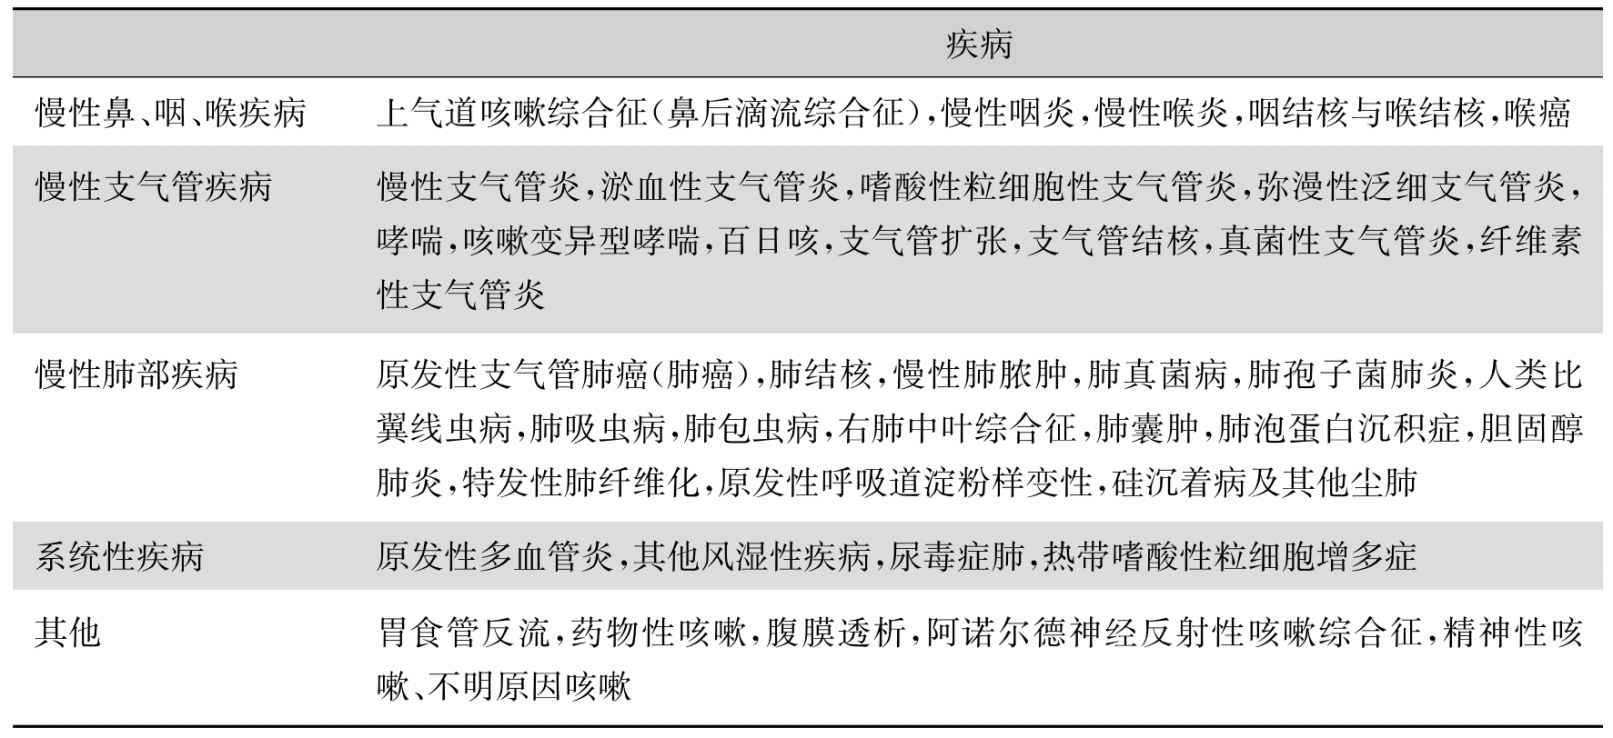
\includegraphics[width=5.90625in,height=2.69792in]{./images/Image00044.jpg}
\end{table}

识别咳嗽的不同特征有助于诊断,包括什么时候开始咳嗽?咳嗽是日间重抑或夜间重?多痰或干咳?痰液的性状如何以及咳嗽伴随什么症状?

健康状态良好的慢性咳嗽,多见慢性咽、喉炎及支气管炎,也可见于支气管扩张。经常作咽部清除动作的咳嗽和咳出黏痰,尤其起床后出现者,多为上气道咳嗽综合征(upper
airway cough
syndrome,UACS)。间歇性咳嗽伴有喘息者多为支气管哮喘。如果每年都在同一时间发作的咳嗽,可能为过敏性鼻炎。日间高声干咳,引起虚脱,伴有情感性反应者提示心因性咳嗽。呈进行性消瘦的慢性咳嗽患者,须注意为消耗性疾病,如肺结核、肺部恶性肿瘤等。

反复咳出大量脓痰者常为肺脓肿,这些患者每有醉酒、昏迷或肺部急性炎症感染病史。如于童年起病,脓痰在经过中逐渐增多,多见于支气管扩张。肺脓肿和支气管扩张的排痰量与体位改变有一定关系。伴有血痰的慢性咳嗽多见于肺结核、肺癌、支气管扩张、慢性肺脓肿、肺吸虫病、淤血性支气管炎等,有时也可见于慢性支气管炎。干咳有服用血管紧张素转换酶抑制剂(ACEI)者要注意药物诱发的咳嗽。

伴有胸痛的慢性咳嗽,常见于肺部病变波及胸膜或附近骨膜,如肺结核、支气管肺癌等。难以忍受的胸部闷痛,须注意支气管肺癌的可能。

长期与有害粉尘接触的慢性咳嗽患者,须注意尘肺的可能性。仰卧时突然发生咳嗽,口腔伴有酸味者提示胃食管反流。

细致的体格检查对60\%病例有诊断价值。体检可发现:咽充血,黏膜可伴有或没有炎性肿胀和脓性分泌物,见于鼻窦炎、上气道咳嗽综合征或过敏性疾病。双肺弥漫性吸气性湿啰音见于肺水肿或肺纤维化。呼气性哮鸣音,见于哮喘或慢性阻塞性肺疾病。散在的湿啰音咳嗽后改变或消失者见于支气管炎。固定的局限性湿啰音见于支气管扩张。肺尖部局限性小湿啰音常提示浸润性肺结核。局限性上肺野大、中湿啰音常提示空洞性肺结核。慢性咳嗽伴杵状指须注意支气管扩张,慢性肺脓肿,慢性肺性骨关节病,特发性肺纤维化。伴颈部及锁骨上淋巴结肿大须注意肺结核、肺癌。

\section{(二)痰检查}

纤维素性支气管炎痰中出现树枝状管型物。痰的细菌学检查(涂片、培养、PCR)对慢性气道和肺部炎症、肺结核、肺真菌病等的诊断有重要意义。痰细胞学检查发现癌细胞能明确肺癌的诊断,痰发现嗜酸性粒细胞增高是诊断嗜酸性粒细胞支气管炎(eosinophilic
bronchitis,EB)的主要指标。

\section{(三)器械检查}

\subsection{1.胸部X线透视及摄片检查}

能进一步确定肺部病变的部位、范围与形态,有时也可确定其性质,如肺部炎症、肺结核、肺脓肿、肺癌、肺囊肿、尘肺等。对于肺深部病变,则X线体层摄片、CT、MRI等诊断价值较大。鼻窦X线检查也有助于寻找咳嗽的病因,可以发现鼻窦炎或鼻窦积脓。胸部CT的横断面图像并无影像重叠,可发现X线胸片未能显示的病灶和小病灶,对肺间质性病变,可较早期清晰显示细小结节及网状阴影。

\subsection{2.纤维支气管镜检查}

对慢性咳嗽患者有时是必需的,可发现大气道内炎症、肿物、异物,并可做活检、支气管肺泡灌洗等。喉镜、鼻咽镜对上呼吸道病变的诊断也是必需的。胸腔镜检查对弥漫性肺疾病和胸膜疾病引起的咳嗽有重要的诊断价值。纵隔镜检查对纵隔病变有时也是必需的。

\subsection{3.支气管激发试验和舒张试验}

可诊断咳嗽变异性哮喘和其他气道过敏性疾病。最大呼气流量(PEF)变异率的测定可评价患者的气道功能状态。

\subsection{4.咳嗽敏感性检查}

通过雾化方式使受试者吸入一定量的刺激物气雾溶胶颗粒,刺激相应的咳嗽感受器而诱发咳嗽,并以咳嗽次数作为咳嗽敏感性的指标。常用辣椒素吸入进行咳嗽激发试验。咳嗽敏感性增高常见于AC、EB、GERC。

\subsection{5.24小时食管内pH监测}

可诊断胃食管反流引起的咳嗽。

\protect\hypertarget{text00063.html}{}{}

\section{13 慢性鼻、咽、喉疾病}

\subsection{一、上气道咳嗽综合征}

上气道咳嗽综合征(UACS)最早源于2006年美国胸科医师协会(ACCP)慢性咳嗽指南,用于代替过去文献中所用的鼻后滴流综合征(postnasal
drip
syndrome,PNDS),后者是指由鼻部疾病引起分泌物倒流至鼻后和咽喉部甚至反流入声门或气管,引起以咳嗽为主要表现的综合征。而UACS的定义为由鼻及鼻窦病变引起的以咳嗽为主要症状的综合征,伴或不伴PNDS,是导致慢性咳嗽的重要原因之一,咳嗽常超过8周,其患病率占慢性咳嗽的22.0\%~57.6\%。本病以慢性咳嗽、咳痰为主要临床表现,常伴有打喷嚏、鼻痒、鼻分泌物增加和鼻塞等,可有鼻后滴流感、面部疼痛及嗅觉障碍。常伴有下列体征:清喉动作、咽部黏膜充血、淋巴滤泡增生(可呈鹅卵石样外观)、咽后壁有黏性分泌物附着等。上述临床症状和体征无特异性,基础疾病的确诊尚需进一步检查。

临床诊断需综合基础疾病、咳嗽与相关症状、鼻咽检查及治疗反应进行综合诊断。我国2009年慢性咳嗽指南提出的诊断标准如下:①发作性或持续性咳嗽,以白天咳嗽为主,入睡后较少咳嗽;②鼻后滴流及(或)咽后壁黏液附着感;③有鼻炎、鼻窦炎、鼻息肉或慢性咽喉炎等病史;④检查发现咽后壁有黏液附着、鹅卵石样观;⑤经针对性治疗后咳嗽缓解。

\subsection{二、慢性咽炎}

\subsubsection{(一)慢性单纯性咽炎}

慢性单纯性咽炎是常见的咽部疾病,其突出的症状为刺激性干咳。由于咽部有瘙痒感及不适感,患者常作廓清咽部的动作,且在讲话多时症状更为显著。患者在讲话中,常须中断,并作吞咽动作以减轻症状。

咽部检查可见咽部充血,咽后壁黏膜表面可见许多扩张的毛细血管及少量淋巴滤泡增殖,咽后壁黏膜及腭弓可略增厚,分泌物可能增多,也可在咽后壁黏膜上发现有黏稠的分泌物附着。

慢性咽炎诊断较易,但病因颇多,须明确其病因,才易于防治。慢性单纯性与慢性增殖性咽炎可由急性咽炎反复发作而来,而大多数继发于上呼吸道病变,如鼻炎、鼻窦炎或口腔慢性炎症。有害粉尘、气体的吸入及烟酒过度等,均可为本病的原因。

\subsubsection{(二)慢性增殖性咽炎}

慢性增殖性咽炎的症状与单纯性咽炎相似,但较显著。

咽部检查可见咽部充血、血管扩张、软腭充血,悬雍垂也可充血、水肿,由于淋巴滤泡增殖、互相融合呈现颗粒状。淋巴滤泡增殖常阻塞咽后壁腺管开口,而致腺体分泌淤积扩大,增加了咽后壁肿胀的程度。咽扁桃体肿大可引起咽鼓管口阻塞而产生耳鸣、听力减退。患者的咽反射特别敏感,常易引起恶心。

\subsubsection{(三)慢性萎缩性咽炎}

咽干燥感是此病最突出症状,患者每于饮水后症状减轻。萎缩的黏膜上被覆痂皮时,常导致干咳、异物感及瘙痒感。

咽部检查发现黏膜苍白、干燥、菲薄而光滑,病变较重者,其上覆盖干燥黏液与痂皮。咽肌萎缩,咽腔似甚宽广。

慢性萎缩性咽炎常继发于萎缩性鼻炎,或咽手术、咽部放射性治疗之后。

\subsection{三、慢性喉炎}

\subsubsection{(一)慢性单纯性与增殖性喉炎}

慢性单纯性与增殖性喉炎的症状以声嘶为主,早期常间歇发生,且每于发音较多时出现。如病情加重,声嘶可成持续,但完全失音者尚属罕见。此外,喉部常有瘙痒、灼热、刺痛等感觉,因此患者常作干咳以减轻症状。

间接喉镜检查时,早期(慢性单纯性喉炎)患者喉部黏膜充血,声带丧失其原有色泽,且可见其上分布有扩张的血管,声带上或杓状间隙可见黏性分泌物黏附。病情加重时(即慢性增殖性喉炎),则黏膜呈暗红色,并有明显增厚,声带暗红,边缘肥厚而呈钝圆,发音时常因声带肥厚而闭合不全,喉室带因代偿活动而致增厚,其较重者可掩盖声带的一部分或全部。

\subsubsection{(二)慢性萎缩性喉炎}

此病比较少见,其主要症状为刺激性干咳,有时甚至可引起声门痉挛。咳嗽之后常咳出黄绿色的痂皮,由于咳嗽用力较猛,每使黏膜损破,以致咳出物带有血丝。声音嘶哑常于痂皮在喉中积聚较多时明显,痂皮排出后好转。由于喉肌萎缩,除声音嘶哑外,常显得软弱无力。此外喉部有灼热感及痛感。

间接喉镜检查时,可见黄绿色或黑绿色痂皮,其严重者甚至在气管内也有痂皮发现。

\subsection{四、咽结核与喉结核}

咽结核与喉结核常继发于开放性肺结核。咽结核的早期,常于水肿、苍白的咽峡、软腭或甚至舌根部出现灰白色结节;此时患者只觉咽部不适,至结节破溃形成溃疡后,才出现咽痛与吞咽痛。疼痛常很明显,患者常因此而拒食。溃疡可发生于咽部各处甚至舌部。溃疡发展缓慢、浅表、边缘不整如鼠咬状,其上附有黏液,但底部较清洁,此外患者常有发热、唾液分泌增多、消瘦及咳嗽等症状。

喉结核早期症状每为干咳及轻度声嘶,声嘶往往出现于下午或晚上,随病情加剧而声嘶越加显著,到后期不仅声嘶而且发音无力,形同耳语。喉部因分泌物积聚而常诱发持久的严重咳嗽。喉部及喉咽部疼痛明显,并常反射至耳部。吞咽痛尤剧烈,进食困难的程度较咽结核更为严重。

喉结核患者咽部黏膜显得苍白,间接喉镜检查,早期常见杓状间隙及会厌披裂后部肿胀,有时早期患者也有出现会厌肿胀的;肿胀之处黏膜均苍白,并有黏液附着于杓状间隙。声带甚至喉室带、会厌等处先后出现溃疡,其严重者喉部形态不能分辨。

\subsection{五、喉 癌}

喉癌常出现咳嗽和声音嘶哑等症状。诊断须经专科医生检查。

\protect\hypertarget{text00064.html}{}{}

\section{14 慢性支气管疾病}

\subsection{一、慢性支气管炎}

患者每年咳嗽、咳痰达3个月以上,连续2年或更长,并可除外其他已知原因的慢性咳嗽,可以诊断为慢性支气管炎。如果肺功能检测FEV\textsubscript{1}
/FVC<70\%,则为慢性阻塞性肺疾病(COPD)。引起慢性支气管炎的内因是机体及呼吸道局部抵抗力降低,外因主要是细菌或病毒感染,有害气体、尘埃的吸入,过冷、过热、过于干燥的空气的刺激以及过敏因素等。

慢性支气管炎多见于中年以上,每于冬春季加剧,夏季减轻或缓解。最突出的症状是咳嗽,尤其是清晨醒后较剧,也可在夜间加剧而致影响睡眠,咳出或多或少的脓性黏液痰,有时也可发生小量咯血。可有微热与全身不适。听诊有散在性干啰音与中、小湿啰音,但也可无明显听诊体征,后期往往并发肺气肿,X线检查可见肺纹理增粗与肺气肿等征象。

慢性支气管炎的诊断,主要应用排除法,即排除其他原因所致的慢性咳嗽而确定之。淤血性支气管炎的患者,有器质性心脏病的体征,每于劳动后或夜间平卧时咳嗽增多。支气管内膜结核,常发生于有开放性肺结核病灶的患者,表现为阵发刺激性咳嗽,有时很难制止,常有哮鸣音,痰中带血,痰抗酸染色可发现抗酸杆菌。支气管镜检查有助于诊断。支气管扩张,每以长期咳嗽、反复大量脓痰或咯血为主要症状,胸部CT、必要时支气管造影可确定诊断。长期接触有害粉尘的慢性咳嗽患者,须注意为尘肺的可能。呼吸道真菌病,其临床表现无特殊,多有长期顽固性咳嗽,咳黏稠痰或带血痰。常发生于身体衰弱或长期使用广谱抗菌素、皮质激素的患者,痰真菌检查发现真菌及菌丝,多次培养阳性及动物接种可助确诊。支气管肺癌发病多在中年以上,可有吼哮样刺激性咳嗽,常持续咯血痰,色鲜红或带褐红色,痰可找到癌细胞,胸部X线检查及支气管镜检查有助于诊断。肺吸虫病及肺包虫病,有地区性流行病学供参考,前者痰常呈铁锈色,痰中易发现肺吸虫卵;肺包虫病多见于牧区,胸部X线检查有特殊征象(参见第30节)。

\subsection{二、淤血性支气管炎}

慢性左心衰竭患者由于支气管黏膜长期淤血,常有持久的咳嗽,多在夜间平卧时或活动后加剧。体检发现两侧肺底弥漫性中、小湿啰音。国内曾见文献报道以慢性咳嗽为首发症状的左心功能不全,使用利尿剂作诊断性治疗,用利尿剂后能降低心脏前负荷,较快地解除了肺淤血和支气管黏膜水肿,从而在排尿后的5~10分钟即表现出镇咳效应。慢性心血管疾病的咳嗽,除由淤血性支气管炎引起之外,尚可能由于主动脉瘤、增大的左心房和扩大的肺动脉压迫气管、支气管,或合并支气管感染、支气管肺炎等所致。在诊断淤血性支气管炎时,上述原因须加以排除。

此外,国内曾报道一例以顽固性咳嗽为表现的室性期前收缩,患者室性期前收缩发作时出现刺激性咳嗽,经给予普罗帕酮治疗后咳嗽消失。

\subsection{三、嗜酸性粒细胞性支气管炎}

嗜酸性粒细胞性支气管炎(EB)是1989年由Gibson等首先定义的一种疾病,为一组痰嗜酸性粒细胞增多,对糖皮质激素敏感,但肺功能正常,无气道高反应性(AHR)的证据,最大呼气流量(PEF)变异率正常的非哮喘慢性咳嗽。主要症状为慢性咳嗽,或晨起咳少许黏痰。部分患者对油烟、灰尘、异味或冷空气比较敏感。目前的研究认为EB是不明原因慢性咳嗽的一个重要病因,大约占慢性咳嗽的10\%~20\%。肺功能和诱导痰检查是诊断EB主要的实验室检查。其诊断标准:①慢性咳嗽,表现为刺激性干咳或伴少量黏痰;②X线胸片正常;③通气功能正常,气道高反应性阴性,呼气峰流速日间变异率正常;④痰细胞学检查嗜酸性粒细胞比例≥2.5\%;⑤排除其他嗜酸性粒细胞增多性疾病;⑥口服或吸入糖皮质激素有效。

EB需和一些肺部寄生虫感染性疾病(如肺吸虫)相鉴别,肺部寄生虫感染也可以表现为慢性咳嗽,少数痰中可见到嗜酸性粒细胞增多,但其外周血中嗜酸性粒细胞明显增高,胸片多有异常,吸入糖皮质激素治疗无效而驱虫治疗有效。

\subsection{四、弥漫性泛细支气管炎}

弥漫性泛细支气管炎(DPB)于1969年由日本学者发现,是一种弥漫存在于两肺呼吸性细支气管区域的气道慢性炎症性疾病。至今病因尚不清楚,可能与人种、遗传因素有关。DPB的受累部位主要是呼吸性细支气管以远的终末气道,病理学特点是炎症病变弥漫性地分布并累及呼吸性细支气管壁的全层。突出的临床表现是咳嗽、咳痰和活动后气促。严重者可导致呼吸功能障碍。在有大环内酯类抗生素疗法之前,DPB多数预后不良,5年生存率只有5\%左右,而大环内酯类抗生素疗法(十四元环、十五元环大环内酯)开展以来已提高到95\%。

本病诊断标准:必备条件:①持续性咳嗽、咳痰、活动时呼吸困难;②合并有慢性鼻窦炎或有既往史;③胸部X线可见两肺弥漫性散在的颗粒样结节状阴影或胸部CT可见两肺弥漫性小叶中心性颗粒样结节状阴影。参考条件:①胸部听诊断续性湿啰音;②一秒钟用力呼气容积(FEV\textsubscript{1}
)占预计值百分比降低(<70\%)以及低氧血症(PaO\textsubscript{2}
<80mmHg);③血清冷凝集试验(CHA)效价增高(>1∶64)。确诊:符合必备条件①、②和③加上参考条件中的2项以上;一般诊断:符合必备条件①、②和③;可疑诊断:符合必备条件①和②。

本病近年国内已有报道。需要和本病相鉴别的是一些临床表现、影像学或病理改变相类似的疾病,如COPD、支气管扩张、支气管哮喘、粟粒型肺结核、结节病、癌性淋巴管炎、肺泡细胞癌、纤毛不动综合征、呼吸性细支气管炎伴间质性肺病(RBILD)和慢性外源性过敏性肺泡炎等,X线胸片、高分辨率CT(HRCT)、病理组织学检查等是主要的鉴别手段。也可通过大环内酯类抗生素进行治疗观察。

\subsection{五、咳嗽变异型哮喘}

咳嗽变异型哮喘(CVA)是以咳嗽为其唯一症状的哮喘,患者无发作性的喘息、气急,双肺无哮鸣音。目前发现约6.5\%~57\%的慢性咳嗽的真正原因为CVA。患者常常具有过敏性疾病或哮喘家族史,或同时患有过敏性鼻炎。咳嗽多为刺激性干咳,发作频繁、剧烈,下半夜咳嗽是其特征。可由于上呼吸道感染、运动、冷空气吸入以及过敏原等刺激而诱发并加重。支气管激发试验常阳性,提示气道高反应性,按照支气管炎给予止咳和抗生素治疗无效,而按哮喘给予支气管舒张剂和吸入糖皮质激素治疗可奏效。CVA患者若不能得到及时诊断及治疗,多数可逐渐发展为典型哮喘。

CVA的诊断要点为:①慢性持续性干咳达1~2个月以上,伴有夜间咳嗽或运动性咳嗽,经正规抗生素及止咳祛痰药物治疗无效;②气道呈高反应性;③泼尼松试验阳性或支气管舒张剂能显著改善咳嗽症状;④除外其他导致慢性干咳的病因。

\subsection{六、变应性咳嗽(atopic cough)}

变应性咳嗽是1992年由日本的学者Fujimura首先定义的一种疾病诊断,表现为变应性非哮喘性慢性干咳,支气管扩张剂无效,肺功能正常,无气道高反应性的证据,峰流速变异率正常,抗组胺药或糖皮质激素治疗效果良好。本病与变应性咽喉炎、EB、感冒后咳嗽的关系及异同还有待进一步明确。其主要临床表现为刺激性干咳,多为阵发性,白天或夜间咳嗽,油烟、灰尘、冷空气、讲话等容易诱发咳嗽,常伴有咽喉发痒。

本病目前尚无公认的标准,中华医学会提出的诊断标准可供参考:

(1)慢性咳嗽。

(2)肺通气功能正常,气道高反应性检测阴性。

(3)具有下列指征之一:①过敏物质接触史,②变应原皮肤针刺试验阳性,③血清总IgE或特异性IgE增高,④咳嗽敏感性增高。

(4)排除CVA、EB、UACS等其他原因引起的慢性咳嗽。

(5)抗组胺药物及(或)糖皮质激素治疗有效。

我国的标准与日本相比,不包括诱导痰和外周血中嗜酸性粒细胞增高,其他基本相同。该病与哮喘、CVA、EB鉴别见表\ref{tab5-2}。

\subsection{七、百日咳}

百日咳是常见的小儿急性传染病,病原体为百日咳杆菌,在儿童集体中易发生流行。病初期表现为急性上呼吸道感染症状(卡他期),约1~2周后出现阵发性痉挛性咳嗽(痉咳期),伴以深长的鸡鸣样吸气声,咳嗽约经2~6周而逐渐缓解(恢复期)。有时也迁延较久,甚至达一年以上。得病后可遗留痕迹反射,一年之内再罹患呼吸道疾病而发生咳嗽时,可出现百日咳样咳嗽。

如病儿咳嗽、咳痰久未康复,须考虑陈旧性肺结核病灶再度活动或继发支气管扩张。

\begin{table}[htbp]
\centering
\caption{EB、哮喘、CVA、AC的临床特征}
\label{tab5-2}
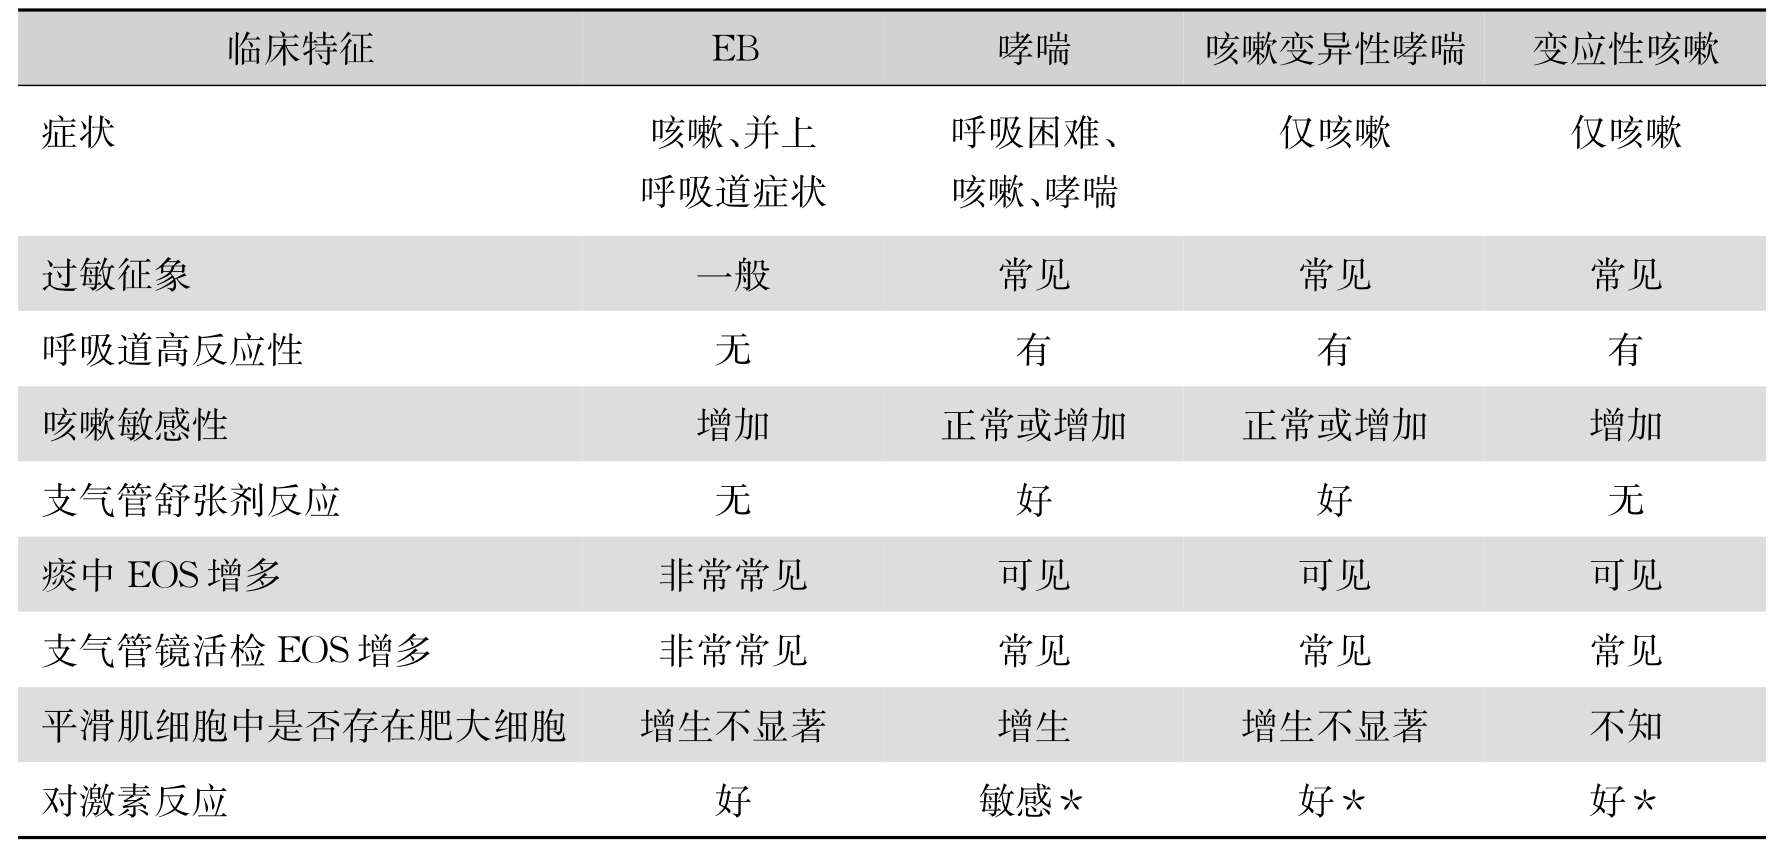
\includegraphics[width=5.9375in,height=2.83333in]{./images/Image00045.jpg}

注:*当痰中EOS增多时
\end{table}



\subsection{八、支气管扩张}

慢性咳嗽是本病的特征之一,干性型支气管扩张患者咳嗽较少,典型者则常咳出大量浆液脓性痰液,并常于晨间或变换体位时咳嗽加剧,患者可有咯血以及同一部位反复发生肺炎(参见第12节)。

\subsection{九、气管、支气管结核}

气管、支气管结核又称支气管内膜结核(EBTB),是指发生在气管、支气管黏膜和黏膜下层的结核病。活动性肺结核中大约10\%~40\%伴有EBTB。主支气管、两肺上叶、中叶、舌叶支气管为好发部位。EBTB起病缓慢,症状多样,缺乏特异性。症状多为咳嗽(刺激性咳嗽为主者较多)、咳痰、低热、盗汗、呼吸困难、体重减轻、咯血(少数病例)、胸痛等;体检少数患者可有肺部局限性哮鸣音、局限性呼吸减弱等;胸片示肺纹理密集、肺纹理粗乱、肺不张、局限性肺气肿等,与慢性支气管炎、肺癌、肺真菌病,甚至支气管哮喘相似,易误诊。有作者报道28例单纯型EBTB(指肺内无结核病灶者)的误诊主要由于:①胸片无结核病灶发现;②胸片虽有肺纹理密集粗乱、局限性肺气肿、叶间胸膜移位等异常,但又非特异性,故未及注意而误诊。

近年的研究提示有下列情况应考虑EBTB的可能:

(1)出现原因不明刺激性咳嗽,反复痰血、呼吸困难、喘鸣和胸部不适。

(2)有下列影像学改变者:①出现变化较快的肺不张、局限性肺气肿;②一侧或两侧肺反复出现支气管播散病灶;③时大时小的张力性空洞或空洞内有气液平面;④肺内无明显病灶,但痰抗酸染色阳性;⑤多部位支气管损害,管腔狭窄、扭曲、变形。周围无明显软组织块影。

(3)纤支镜检查对确诊EBTB有决定性作用。建议对凡有干咳、胸闷、喘鸣、咳黏液痰者,经抗炎、对症治疗2周未见好转时及早作纤支镜检查,镜下刷检涂片染色找抗酸杆菌,及(或)做活检送病理组织检查。如无发现而患者疑似本病时,2周后再做纤支镜刷检抗酸杆菌与活检标本病理检查。目前PCR已用于结核病的病原学诊断,对诊断有进一步帮助。

气管、支气管结核的诊断标准如下:①结核病临床表现及临床治疗反应;②痰涂片、集菌抗酸杆菌阳性,最好是培养MTB阳性;③影像学改变;④PPD试验阳性;⑤支气管镜下直视的气管、支气管典型病变;⑥支气管刷片或支气管冲洗液抗酸杆菌阳性;⑦经支气管镜活检组织提示结核性病理改变。符合具备上述5+6、5+7、5+2为确诊标准,1+2+3、1+3+4、2+3、3+4、5、6、7为高度疑诊标准。

\subsection{十、真菌性支气管炎}

真菌性支气管炎比较少见,常继发于全身衰弱、营养不良的患者,长期接受糖皮质激素与广谱抗生素治疗的患者,接受放射治疗、化学治疗的恶性肿瘤患者,或慢性肺部疾病的患者。但也可原发性发病(参见第17节)。

\subsection{十一、纤维素性支气管炎}

纤维素性支气管炎又名纤维蛋白性支气管炎、管型支气管炎和成型支气管炎等,临床上较少见。病因、病理和发病机制尚未完全清楚,多继发于支气管炎、肺结核、心力衰竭等。目前多认为发病机制与变态反应有关,可能是特异质患者在各种致病因子作用下,呼吸道黏膜发生变态反应,使血管壁通透性增强,炎性物质和纤维蛋白渗出,腺体分泌亢进,细胞浸润聚集于管腔内。在组织凝血酶和黏液酶及管腔内pH值改变的作用下,分泌物脱水、浓缩、凝固,从而铸成支气管样管型。又因机体的排异作用,使管型剥离而损伤小血管,导致咯血。

本病常见的临床表现为咳嗽,可为剧咳或呛咳,管型咯出前有胸闷、气憋或窒息感;咯血,多少不等,一般50~1000ml,咯血前咽部奇痒或咽部有阻塞感;咯出支气管管型,为树枝状膜样管型物,灰白色、淡褐色或浅红色,咯出管型后咳嗽、胸闷、窒息感可迅速缓解。咯出的管型清水漂洗后常可见典型的支气管管型,大体上呈树枝状、膜片状,柔韧性好,不易碎裂。管型一般长约5~6cm,最长可达30cm,主干中空,末端变细,有的呈丝状。镜下检查为红染均质的纤维素,中间混有多少不等的中性粒细胞、嗜酸性粒细胞及淋巴细胞。体检肺部呼吸音减低或可闻及干湿啰音,血象白细胞可轻度增高,合并细菌感染者可显著增高并伴发热。胸部X线检查一般正常,极少数可在肺门区或心缘旁有尖端向内的楔形或Y形阴影或表现为局限性肺不张,但均无特异性诊断价值。纤支镜检查可发现附着于气管或支气管的管型,有助于诊断。

\protect\hypertarget{text00065.html}{}{}

\section{15 慢性肺部疾病}

\subsection{一、原发性支气管肺癌(肺癌)}

原发性支气管肺癌简称肺癌,指肿瘤细胞源于支气管黏膜或腺体。肺癌按解剖学部位可分为中央型肺癌和周围型肺癌,前者发生在段支气管至主支气管,约占3/4,以鳞状上皮细胞癌和小细胞未分化癌较多见;后者发生在段支气管以下,约占1/4,以腺癌较为多见。肺癌按组织病理可分为非小细胞肺癌(NSCLC)和小细胞肺癌(SCLC),前者包括鳞状上皮细胞癌(鳞癌)、腺癌、大细胞癌、腺鳞癌、类癌、支气管腺体癌等;后者包括燕麦细胞型,中间细胞型、复合燕麦细胞型。

早期肺癌大多无症状或体征,当出现以下临床表现时应警惕肺癌的可能,尤其是对于40岁以上有长期吸烟史(吸烟指数>20包年)者,应尽快行胸部影像学检查明确:

1.持续性无痰或少痰的刺激性咳嗽,或原有慢性咳嗽的性质发生改变。

2.咯血或痰中带血。

3.气短或喘鸣,听诊时可发现局限或固定性哮鸣音。

4.发热,抗生素治疗效果不佳。

5.体重下降。

6.同一部位反复发生肺炎。

7.出现原因不明,久治不愈的肺外征象,如杵状指(趾)、非游走性肺性关节疼痛、男性乳腺发育、皮肤黝黑或皮肌炎、共济失调。

8.出现局部侵犯及转移的体征,如声带麻痹、上腔静脉压迫综合征、Horner综合征、Pancoast综合征、锁骨上窝淋巴结肿大等。

肺癌的诊断,主要采取综合诊断方法。

胸部X线检查普及率广、应用方便、辐射量小,但分辨率低,不易检出肺内隐蔽部位病灶和微小病灶,在早期肺癌的检出应用方面有一定局限性。早期肺癌的X线征象主要有以下几种:

1.局限性肺气肿
支气管内极小的癌瘤,X线检查常无异常发现,当肿瘤长大引起支气管部分性阻塞,空气入易出难,则在阻塞远端的肺组织形成局限性肺气肿。局限性肺气肿是肺癌早期征象之一。在透视或摄片时作呼气检查,较易观察到肺气肿部分与其他部分肺脏的对比。

2.肺不张
肿瘤完全阻塞支气管时则引起肺不张。临床上发现年龄较大的肺不张患者,应考虑肺癌的可能性。

3.一侧肺门阴影增宽
此种阴影是由癌、淋巴结肿大及癌周围组织炎症病变所构成,边缘多呈毛刺状,是中央型肺癌最常见的X线征象。如有淋巴结转移,可认为是较晚期的表现。

4.孤立性结节阴影
早期的周围型肺癌常呈小的圆形或椭圆形结节阴影,边缘常不整齐,常凹入或分叶状;结节阴影绝大多数为单发性。如为大小相似的多发性阴影,大概不是原发性肺癌(参见第31节)。

5.不消散的或反复出现的节段性肺炎。

当肺癌在支气管内继续生长和分泌物引流受阻时,则可引起阻塞肺段的局限性肺炎。此种肺炎虽经积极的抗生素治疗仍不消散。

肺癌的早期诊断还须依靠下列检查:

\subsubsection{1.痰细胞检查}

痰液脱落细胞检查是目前诊断肺癌简单方便的无创伤性诊断方法之一,连续三天留取清晨深咳后的痰液进行痰细胞学涂片检查可以获得细胞学的诊断。液基细胞学可以提高诊断率。高质量的痰标本和标本优化处理是提高细胞学检查阳性率的重要保证。有报告阳性率可达80\%,其优点是不致增加患者的痛苦,易于接受。可嘱患者清晨漱口后,用力咳出第二、三口痰立即送检。阴性时反复多次送检。

\subsubsection{2.纤维支气管镜检查}

可直视下刷检或(及)钳夹活检,或透视指导下经纤支镜肺活检,或经支气管针刺吸引活检。目前应用荧光支气管镜和超声支气管内镜技术(EBUS)对支气管内病变组织及支气管周围肿大淋巴结的活检提高了肺癌的诊断率。

\subsubsection{3.CT和PET/CT}

是一种无创伤性检查方法,患者易于接受,可检出早期肺癌,是目前诊断肺癌的重要手段。可以提示病变所在的部位和累及范围,可为区分其良恶性提供重要参考意见。对肺内病灶,特别是纵隔和心影后的病灶,CT检查可比X线检查显示较清楚的影像。低剂量CT(LDCT)可以有效地发现早期肺癌,已经逐步取代胸片成为较敏感的肺结节评估工具。美国胸外科学会推荐对年龄在55~79岁、吸烟指数达30包年的成人每年进行低剂量螺旋CT进行肺癌筛查,而对于吸烟指数达20包年且预计5年累积肺癌发生率在5\%以上的成人,筛查起始时间应提前至50岁。

\textsuperscript{18}
F-脱氧葡萄糖(F-18fluoro-deoxyglucose,FDG)正电子发射断层显像(positron
emission
tomography,PET)正电子断层扫描仪将人体代谢所必需的物质如葡萄糖、蛋白质、核酸、脂肪酸等标记上具有正电子放射性的短寿命核素,制成显像剂(如氟代脱氧葡萄糖)注入人体后进行扫描成像。放射性\textsuperscript{18}
FDG注入体内后,肿瘤组织对其摄取率明显增加,从而被探测系统记录,经计算机图像重建显示三维断层图像。因此,PET有助于胸片或CT检查发现病变的定性诊断,以及肺癌治疗前后的疗效判断。有学者报道PET用于CT不能定性的病变诊断肺癌的敏感性高达95\%。PET可以弥补螺旋CT定性困难的不足。该检查有助于无创性鉴别良恶性结节,甚至还可为选择病灶进行活检或穿刺检查提供重要参考意见,在高代谢的病灶处活检更容易获得可靠的结果。但鉴于其价格昂贵,不推荐作为常规检查。对5mm以下的病灶或磨玻璃样阴影其诊断价值受到限制。

\subsubsection{4.磁共振显像(MRI)}

是一种非侵入性检查,已用于肺癌的诊断。它与CT二者各有优点,可互相补充。CT能全面地显示病灶范围,但对中心型小结节,有时易误认为肺血管断面,而MRI观察血管有良好的天然对比(流空效应),故可鉴别肺门或纵隔内的肿物是否为血管性或非血管性。MRI较增强CT更好地显示肺门及纵隔内的淋巴结和肿块,但CT在检测气管及支气管病变方面则优于MRI。

\subsubsection{5.其他器械检查}

近年来,更多的检查用于肺癌的诊断,包括单光子发射计算机断层扫描(SPECT)、经胸壁细针穿刺活检、纵隔镜检查、胸腔镜检查、开胸肺活检等,可根据需要选用。

\subsubsection{6.血清肿瘤标志物检查}

目前尚无特异性肺癌标志物应用于临床诊断,但部分标志物可作为肺癌诊断或者评估肺癌治疗效果的参考。如在随访阶段发现肿瘤标志物水平进行性升高,需积极进行下一步检查。现阶段,常用的血清肿瘤标志物有以下几种:

\paragraph{(1)癌胚抗原(carcinoembryonic antigen,CEA):}

主要用于肺癌诊断和判断预后以及对治疗过程的监测。

\paragraph{(2)细胞角蛋白片段19(cytokeratin fragment,CYFRA21-1):}

对肺鳞癌诊断的敏感性、特异性有一定参考意义。

\paragraph{(3)鳞癌抗原(squamous cell carcinoma antigen,SCC):}

对肺鳞癌疗效监测和预后判断有一定价值。

\paragraph{(4)神经元特异性烯醇化酶(neuron specific enolase,NSE):}

用于小细胞肺癌的诊断和治疗反应监测。

\paragraph{(5)胃泌素释放肽前体(pro gastrin releasing peptide,Pro-GRP):}

可作为小细胞肺癌的诊断和鉴别诊断的首选标志物。

如患者临床未能排除肺癌,而上述检查阴性,仍须定期作X线胸片与痰中癌细胞检查。对病因未明的反复的或持久性节段性肺炎与肺不张,或周围性结节状病灶无法排除肺癌时,可考虑开胸探查。抗结核的诊断性治疗,一般不应超过4周,以免错过手术根治的机会。

多数作者认为,有症状的肺癌往往已属晚期,无症状者(隐性肺癌)常属早期,故应重视亚临床、无症状病例的发现。对高发区人群和长期吸烟者尤须作定期的普查,以期无症状早期肺癌的发现。

肺癌误诊病例不少,特别是早期肺癌,主要由于:①因年龄在30~40岁以下而不引起注意,致误诊为肺结核、支气管扩张、节段性肺炎等;②由于胸腔积液为浅黄色浆液性,或为包裹性积液而误诊为结核病;③由于有多关节炎症状而误诊为类风湿关节炎或风湿性关节炎;④由于血性心包积液而误诊为原发性心包炎等。偶尔早期肺癌在X线胸片上被肋骨掩盖而致漏诊。

如肺癌引起淋巴结转移、血性胸腔积液、Horner综合征或其他器官(肝、骨、脑、肾等)的转移,则已属晚期现象。

\subsubsection{(一)细支气管-肺泡细胞癌}

细支气管-肺泡细胞癌女性较多见,半数以上有咯血,有较为特别的临床与病理学表现。癌多于肺的边缘生长,不侵犯大支气管。症状发展缓慢渐进,以咳嗽、咳痰、气短较常见。痰量可能甚多,有时可达数百毫升,是与一般早期肺癌不同之点。此型肺癌可有不同程度的炎症、坏死,但极少形成空洞。体征因癌瘤的大小与位置而定,一般较易引起胸腔积液。X线检查可分孤立结节型、弥漫型、肺炎型三种表现,以孤立结节型最多见。由于不同的X线表现,易与肺结核、肺炎、支气管扩张、慢性支气管炎、胸膜炎等相混淆。

细支气管-肺泡细胞癌可有下列临床表现供诊断参考:①病情发展缓慢,自起病至确诊可能经过半年以上;②肿瘤位于肺的外周部分,早期即累及终末支气管与胸膜;③患者每有呼吸困难等缺氧现象;④由于癌细胞可分泌黏液,因而有顽固性咳嗽和咳出大量黏稠、胶冻样的痰液,是部分患者突出的症状。

此型肺癌在支气管造影片上有下列征象:①受累的支气管呈均等而明显的狭窄;②支气管影像呈僵硬、伸长;③造影剂充盈于支气管内而不黏附在壁上;④因支气管的细小分支和肺泡不充盈,所以支气管树呈枯枝状。痰内癌细胞检出率高,有重要诊断意义。又因此型癌细胞易于剥落,支气管肺泡灌洗液沉渣中较易检出癌细胞。

弥漫型细支气管-肺泡细胞癌与急性粟粒型肺结核的X线表现相似,临床上常导致误诊,两者的鉴别可参考表\ref{tab5-3}。

\begin{table}[htbp]
\centering
\caption{弥漫型细支气管-肺泡细胞癌与急性粟粒型肺结核的鉴别}
\label{tab5-3}
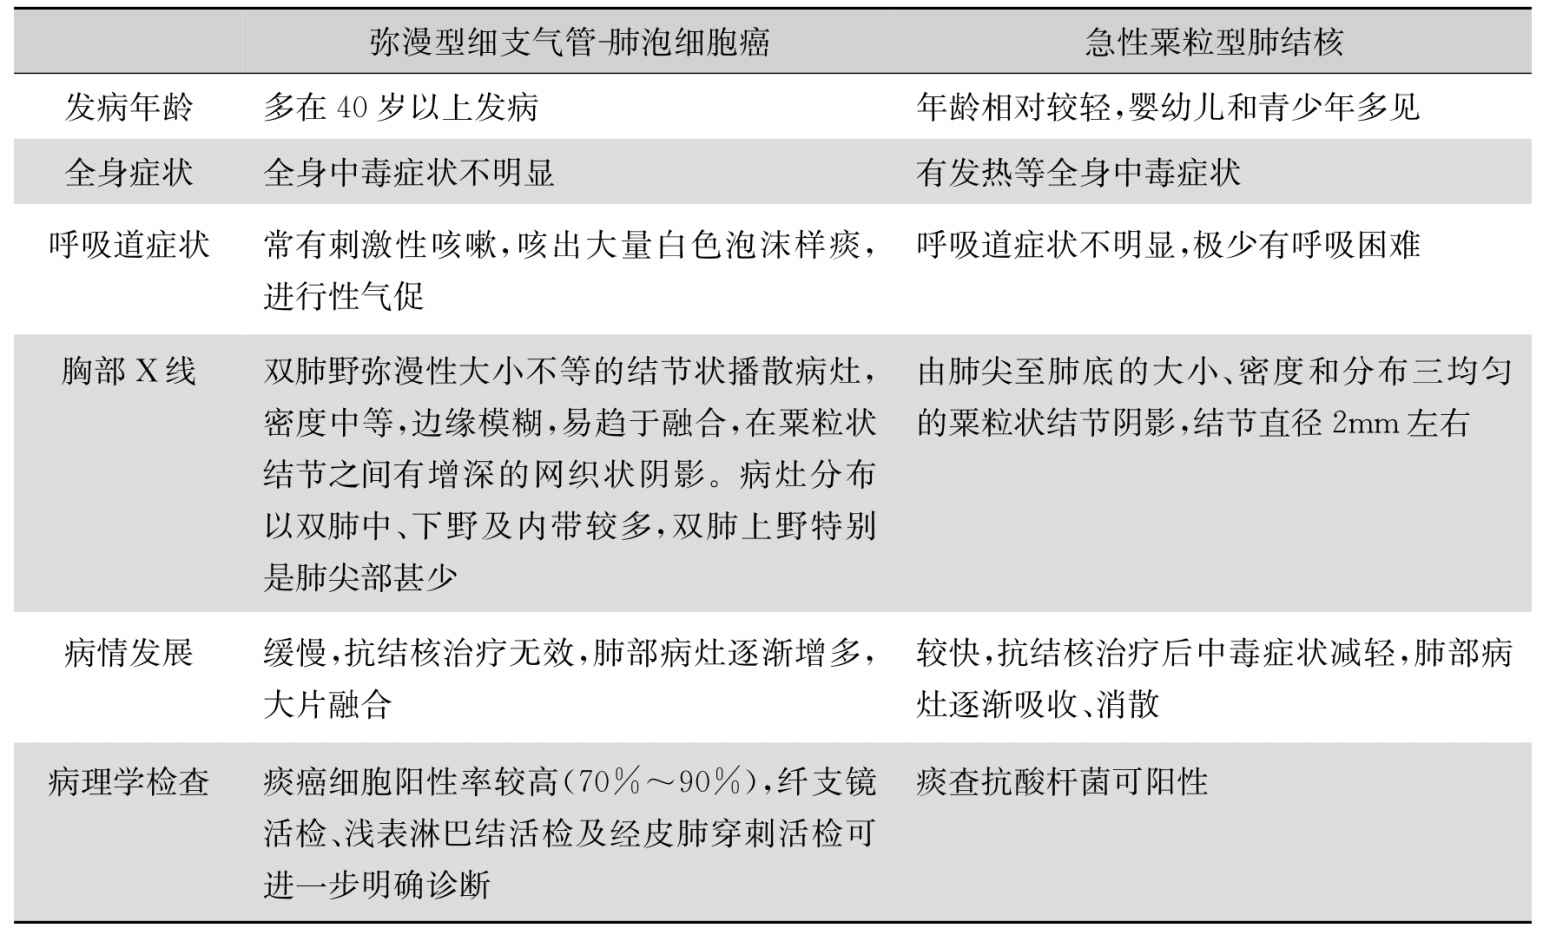
\includegraphics[width=5.91667in,height=3.58333in]{./images/Image00046.jpg}
\end{table}

\subsubsection{(二)肺瘢痕癌}

肺瘢痕癌少见。患者多以胸痛、咳嗽、气短、痰中带血为主诉。先期存在的肺瘢痕组织成因多种多样,如尘肺、结核、慢性炎症、支气管扩张、囊肿、异物、梗塞等,尤其以肺结核瘢痕灶的基础上发生的瘢痕癌病例多见。国内报告术后无长期生存的病例。对于肺部有呼吸系统疾病史同时伴有瘢痕形成者,应定期予胸部CT复查、随访。当发现病灶大或密度增高、不均匀,边缘由光整变为不规则甚至出现毛刺、分叶者,应考虑瘢痕癌,必须进一步检查以明确诊断。

\subsubsection{(三)支气管类癌}

少见,主要表现为咳嗽、咯血、发热和反复发作的肺炎。具有发病年龄轻、生长慢、恶性度低、较少转移的特点。应注意与肺癌、结核球及良性肿瘤鉴别。参见第12节。

\subsection{二、肺结核(参见第12.2节)}

\subsection{三、慢性肺脓肿}

急性肺脓肿3个月后未愈,称为慢性肺脓肿,如脓肿周围发生纤维组织增生,常继发支气管扩张。痰量常较多,常有腐臭气味,静置后可分为三层:上层为泡沫;中层为水样浆液层,常为淡绿色;下层为脓层,含有坏死的细胞和碎屑。临床症状往往好转与恶化交替,在间歇期中患者自觉较良好,在恶化期间则症状加重,体温升高,咳嗽,痰量增多,胸痛加剧,血象白细胞增多,并可出现杵状指及肺性骨关节病,内脏(肾、肝)淀粉样变性,贫血和低血浆蛋白性水肿等。

慢性肺脓肿常伴有脓腔周围继发性支气管扩张,须与原发性支气管扩张区别。晚期的支气管扩张也可形成多发性小脓肿,症状与肺脓肿相似。支气管扩张患者常有多年咳嗽、反复咯血和多痰的病史,体检时病变部位可听到多数固定性湿啰音,X线检查可发现支气管卷发样阴影或多发性管状小空腔,胸部CT检查显示管壁增厚的柱状扩张或成串成簇的囊状改变。慢性肺脓肿又须与癌性空洞区别,如经积极抗菌药物治疗,局部支气管阻塞仍未缓解,X线征无好转,空洞壁厚而内缘不规则,呈偏心性,须疑为肺癌,如伴有肋骨骨质破坏则肺癌的诊断大致可以确定。慢性纤维空洞性肺结核也易被误诊为慢性肺脓肿;结核性空洞多位于上肺,空洞内多无气液平面,周围常有结核播散形成的卫星样病灶,一般易于区别。也有少数肺脓肿患者发病不急,痰少,就诊时血象白细胞正常,或呈孤立性空洞,或短期内对青霉素无效,难与结核性空洞鉴别。但肺脓肿病史较短,感染症状比较明显,脓痰多或有臭味。改用有效的抗菌药物可显著好转,慢性病例常发生杵状指或肥大性骨关节病等,痰菌检查有助于二者的鉴别。右下肺脓肿须注意阿米巴肺脓肿的可能,如表现较重的中毒症状,咳棕褐色痰,应怀疑肺阿米巴病,在痰液或脓液中找到溶组织阿米巴或经抗阿米巴治疗奏效可确定诊断。

\subsection{四、肺奴卡菌病}

奴卡菌为放线菌科中的一个属。自从糖皮质激素与免疫抑制剂广泛应用以来,肺奴卡菌病有增加的趋势,国内也有少数病例发现。73\%的奴卡菌病初发于肺脏,可无症状,但多有咳嗽,咳痰、咯血痰、胸痛、脓胸(占20\%)等症状,常伴有发热、乏力、食欲减退、消瘦等全身症状。X线表现无特异性,可有肺炎样、多发性结节、肺脓肿、空洞形成、胸腔积液、粟粒样病灶等征象。易发生血行播散性感染。诊断须根据患者致病诱因、上述临床及X线表现,以及痰、胸腔积液或血培养中证明有奴卡菌存在,以及除外其他原因的肺部病变而确定。

\subsection{五、肺放线菌病}

肺放线菌病国内报告例数不多,发病通常徐缓,开始表现为支气管炎症状,患者有咳嗽,咳黏液痰。当感染侵入肺部引起肺炎或脓肿时,症状加重,咳脓痰或血痰、伴有寒战、发热。可累及胸膜及胸壁。此病的临床症状、体征和胸部X线征象并无特异性,因而早期诊断不易,常被误诊为肺结核、结核性胸腔积液、肺脓肿或肺癌等。如对上述疾病在诊断上有所怀疑,对本病有所警惕,而进行真菌检查,可在痰中或胸腔积液中找到“硫磺颗粒”及培养出放线菌。

此病后期损害肋骨,产生胸壁脓肿及胸壁瘘管形成,此时诊断则较易。在瘘管分泌物中也可找到“硫磺颗粒”及放线菌。

\subsection{六、肺真菌病}

目前在我国常见的肺真菌感染,其致病菌最多为白念珠菌与曲霉,其次为新型隐球菌。此外国内文献还有少数的肺毛霉病报道。前两种多以寄生形式存于人体内,在一定条件下继发呼吸道感染,而新型隐球菌则以原发性致病多见。呼吸道真菌病的临床表现多无规律性,肺部X线表现也形态不一,易侵犯胸膜,可通过血道、淋巴道侵犯神经系统或引起全身播散,常被误诊或漏诊。

临床上有下列一些表现时须考虑肺部真菌病的可能性:

1.老年、幼儿或体弱、营养不良的患者,长期接受广谱抗生素、糖皮质激素、放射线照射或抗肿瘤化学治疗的患者,器官移植患者,病程中出现肺部感染病征。

2.慢性呼吸道疾病如慢性支气管炎、慢性阻塞性肺疾病、支气管扩张、肺结核、慢性肺脓肿等经积极的抗菌药物治疗无效,或病情反而加重者。

3.肺部X线摄片呈粟粒状、斑片状、大片状或圆形块状阴影,而这些病变无特征性改变,即不似肺结核、炎症、肿瘤、寄生虫病等,经抗炎症、抗结核治疗无效或病变反而加重者。

4.经常与家禽、牲畜、稻草、土壤接触或从事酿酒工作,而出现病因未明的肺部病变者。

5.胸壁脓肿、肋骨损害及胸壁瘘管形成。

\subsubsection{(一)肺白念珠菌病}

白念珠菌常侵犯支气管和肺。此种真菌常寄生于正常人的上呼吸道、消化道和皮肤上,感染常为内源性,并在上述1、2两项的致病条件下,使真菌有机会在支气管内繁殖,并进一步侵入肺内。其病程可为急性、亚急性和慢性。

症状比较复杂,一般是慢性进行性,有顽固性咳嗽,咳痰。痰的特点是量少,胶样黏稠或带有乳块状或血丝,如夹杂细菌感染则为脓样。常有发热(38~39℃)、疲乏、盗汗、脉快、纳差、呼吸困难、胸痛等症状。体检所见与其他慢性肺部感染难以区别,可出现啰音、肺实变征、肺空洞与胸腔积液征。此病可与支气管扩张、肺结核、肺脓肿、肺癌等并存。

肺白念珠菌病有下列X线征象:①斑片状阴影;②大片状阴影;③粟粒状阴影;④胸腔积液;⑤肺门淋巴结肿大,肺纹理增多;⑥空洞形成,钙化现象等。

肺白念珠菌病的诊断主要根据:①在无污染的痰液(通常嘱患者早上刷牙后用1\%双氧水含漱10分钟,继用清水漱口,用力咳嗽,弃去第一口痰液、留第二、三口痰液立即送检),或纤支镜检采得的分泌物(此法取材可靠),或胸腔抽出液,多次培养分离出纯种的白念珠菌落,或胸膜活组织病理检查证明有此菌;②临床与X线检查符合此病的表现;③除外肺结核、肺肿瘤、肺脓肿及其他真菌感染(但也可与之并存);④停用抗生素与糖皮质激素,改用抗真菌治疗,有较好的疗效。

\subsubsection{(二)肺曲霉病}

曲霉在自然界分布甚广,一般认为与发霉的谷草、家禽(如鸡、鸭、鸽)、牲畜(牛、羊、马)等接触及酿酒等工作可得此病。肺曲霉感染可以继发于上述1、2两项的致病条件下。

肺曲霉病主要由烟曲霉引起,临床上主要有五种类型:侵袭性肺曲霉病、气管支气管曲霉病、慢性坏死性肺曲霉病、曲霉肿和变应性支气管肺曲霉病(ABPA)。参见第3.1.7节。

起病可急可缓,临床表现多为慢性咳嗽,反复咯血,症状和X线表现可多种多样。侵袭性曲霉病X线特征性改变是以胸膜为基底的多发的楔形阴影或空洞,胸部CT早期的典型表现为晕轮征(halo
sign),后期为新月体征。曲霉肿表现为空洞内有可移动的团球影(曲菌球)。ABPA为上叶短暂性实变或肺不张,中央支气管囊状扩张及壁增厚征象如“戒指征”或“轨道征”。

肺曲霉病临床表现大致可区分为:①类似肺结核、肿瘤或肺脓肿的表现,X线胸片可呈现圆形阴影,有时与肺结核球、肺结核空洞、肺包虫病、肺脓肿不易区别;②反复咯血或咳出大量的泡沫痰(可带有酒味),类似支气管扩张;③急性经过类似大叶性肺炎或小叶性肺炎;④气喘发作类似喘息性支气管炎;⑤全身性多发性小脓肿,呈败血症的病象。

肺曲霉病的诊断主要根据:①有与曲霉接触的职业史。②有上述临床症状和X线改变。③真菌学检查:咳出的深部痰连续三次直接镜检见曲霉丝及芽孢,且培养得到同一型的曲霉支持肺曲霉病的诊断。病理活检发现菌丝及组织培养得到曲霉是确诊的“金标准”。④除外肺结核、肺脓肿、肺癌、支气管扩张及肺炎等疾病,但须注意肺曲霉感染也常继发于上述疾病的基础上而与之并存。⑤抗真菌药治疗有一定的疗效。

\subsubsection{(三)肺隐球菌病}

肺隐球菌病是由新型隐球菌感染引起的一种亚急性或慢性肺部真菌病。主要见于成人,约50\%患者为免疫功能正常的宿主。隐球菌病以中枢神经系统感染最为常见,其次为肺部。一般认为此病首先累及肺部,如果宿主自身免疫力低下,隐球菌不能局限在肺部,就有可能发生全身播散。临床上单独肺部受累的隐球菌病并不多见,仅占全部隐球菌病的13\%~20\%。

本病多无症状,少数患者有干咳、咳少量黏液痰或血丝痰,咯血比较少见,常伴有胸痛、微热、乏力等症状。如有广泛性感染,则出现肺实变体征。本病的影像学表现多样,可呈:①孤立性块影:直径约2~7cm,多见于原发性肺隐球菌病(占81\%);②大片致密影伴小透亮区;③单发或多发性结节影;④单发或多发性斑片状浸润影:常为继发性肺隐球菌病;⑤弥漫性粟粒影;⑥间质性肺炎型:此型少见。⑤⑥常见于免疫功能低下者。另外也可表现为空洞、胸腔积液及肺门淋巴结肿大。影像学的表现无特异性,易与肺癌、肺转移性肿瘤、肺结核、Wegener肉芽肿等疾病相混淆,尤其是孤立性块影与肺癌不易鉴别。

肺隐球菌病的确诊可依靠痰、胸腔积液、支气管肺泡灌洗液、纤支镜病灶刷片、经皮肺穿刺涂片、脑脊液直接涂片加墨汁于光镜下检查;经纤支镜肺组织活检、经皮肺穿刺活检是有价值的确诊手段;间接免疫荧光法在血液中可找到隐球菌循环抗体;必要时行胸腔镜或开胸活检。

\subsubsection{(四)肺毛霉病}

对有免疫功能缺陷的患者,出现呼吸道症状时,须考虑肺毛霉病的可能。临床与X线胸片均无特征性表现。X线表现不一,可为结节状影、多发性小斑片状阴影、肺炎样改变、空洞形成、胸腔积液等。反复做痰、胸腔积液等检查,必要时做肺活检,发现大量毛霉,并除外其他原因的肺部疾病,即可确定诊断。

\subsubsection{(五)肺孢子菌肺炎}

卡氏肺囊虫以前归类为原虫,目前认为是真菌,并命名为孢子菌,侵犯人体的主要为耶氏孢子菌。主要侵犯早产儿和先天性或获得性免疫功能缺陷的人,导致条件致病性感染。健康人偶可罹患。病变绝大多数局限于肺部,主要临床表现为干咳、进行性呼吸困难、发绀,部分患者有发热。呼吸系统症状虽重,但肺部体征甚少或全无,即症状和体征分离,少数患者有肺底湿啰音。淋巴结、肝、脾可肿大。对免疫功能缺陷患者出现上述症状时,应考虑本病之可能。痰及支气管灌洗液中病原体阳性率不高。开胸活检阳性率最高,可达95\%,但并发症多,危险性大。血清特殊性免疫学检查有重要诊断价值。痰和血PCR检测对诊断亦有良好价值。参见第3.1.7节。

\subsection{七、肺寄生虫感染}

\subsubsection{(一)肺(胸膜)阿米巴病}

参见第3.1.8节。

\subsubsection{(二)人类比翼线虫病}

本病亦称喉比翼线虫感染,大多数患者表现为慢性咳嗽。如成虫侵蚀支气管壁,则可引起咳血痰或咯血。咯血多为少量。体重减轻常见。也有咳出鲜红色的Y形线虫而确诊。X线胸片无特异性,可表现为支气管炎或肺炎。广州曾报道三例,一起进食龟后发病,均未到过国外,可认为国内感染,纤支镜下钳出此虫而得确诊。

\subsubsection{(三)肺吸虫病}

肺吸虫病患者都有咳嗽与咳痰,且常为早期症状,痰一般为白色黏性,如继发感染则呈黄色脓性,而锈色痰是本病特征之一(参见第12.2节)。

\subsubsection{(四)肺包虫病}

参见第30节。

\subsection{八、右肺中叶综合征}

右肺中叶综合征是由右肺中叶支气管本身病变或管腔受压狭窄,引起右肺中叶膨胀不全或不张,肺叶体积缩小的临床综合征。患者最常有的主诉为慢性咳嗽、咳痰、胸痛、发热及咯血等。如患者有反复发作的右中叶肺炎病史,右前胸中部呈实变体征,须考虑此综合征的可能。其诊断根据是:①右中叶肺不张;②阻塞性肺炎;③受压支气管狭窄;④右叶支气管旁淋巴结肿大。胸部X线检查、CT扫描及纤支镜检查对诊断有重要帮助。

成人右肺中叶综合征可发生于任何年龄与性别,但以21~30岁为多。最常见的病因为肺部炎症、恶性肿瘤和结核,其他的病因有淋巴结炎、结节病、尘肺、真菌病、支气管扩张、支气管结石、囊肿、脓痰栓、外伤、寄生虫、异物等,导致支气管狭窄或右肺中叶支气管淋巴结肿大,压迫支气管,形成压迫性肺不张,导致阻塞性肺炎及受压部位之下的支气管扩张。胸部X线照片是可靠的诊断方法。纤支镜检查可直接窥视右肺中叶开口病变的情况,支气管造影可了解支气管病变的程度与受压情况。

\subsection{九、肺囊肿}

肺囊肿与支气管沟通则易继发感染。如有继发感染,则出现咳嗽、咳痰、发热及小量咯血等症状。肺囊肿可分为先天性及后天性两种,以前者为多见。先天性肺囊肿系因胚胎时期某一部分肺芽发育障碍,不能形成管状,其远端支气管所分泌的黏液不能排出,逐渐积聚膨胀成为囊肿。先天性肺囊肿较多在儿童期出现症状。后天性肺囊肿多因肺部炎症后,肺泡壁损害,加以小支气管黏膜因炎症使管腔部分阻塞呈活瓣样作用,空气入易出难,肺泡内压力增高而形成。多发性先天性肺囊肿常伴有支气管扩张,症状与支气管扩张相似,由于病变多位于中、上肺,引流较易,较少引起发热。X线胸片检查呈圆形透亮影,其壁菲薄而整齐;多发性者大小不一,可分布于任何肺野,但以中、上肺野较多见。

先天性肺囊肿的诊断主要根据幼年发病史、上述的临床表现以及胸部X线摄片(正位与侧位)检查。胸部CT检查对诊断也有较大帮助。

多发性先天性肺囊肿须与支气管扩张鉴别,可根据下列几点:①肺囊肿多位于上肺,痰液引流较通畅,症状较轻;支气管扩张多位于下叶,痰液易于潴留而炎症症状往往较明显;②肺囊肿常为多发性,圆形,大小可相仿;支气管扩张管腔多呈囊状或圆柱状扩张,管腔大小相差较悬殊;③肺囊肿与支气管扩张的病变范围虽常为多支段性,但肺囊肿除为多支段性外,往往也为多叶性,发病部位并无规律性;④多发性肺囊肿在X线平片上于病侧可有肺气肿与肺大疱的征象,而支气管扩张则少有这些征象。

肺囊肿继发感染时可出现大片模糊阴影,类似浸润性肺结核,但经抗生素治疗后感染较快消退,而有别于肺结核。

肺囊肿有时须与肺脓肿相区别。囊肿合并感染时,其临床症状和X线改变类似肺脓肿。肺囊肿的囊外浸润比肺脓肿少,囊内液体较多,与囊外浸润不成比例;炎症吸收后,可出现薄壁囊腔。

\subsection{十、肺泡蛋白沉积症}

肺泡蛋白沉积症(PAP)是指肺泡和细支气管腔内充满不可溶性的富磷脂蛋白质物质的疾病。PAP属于少见病,好发于青中年,男性患病率约为女性的2倍,病因未明,可能与感染因素、肺表面活性物质清除异常、肺泡巨噬细胞功能缺陷或吸入有害气体或粉尘有关。发病大多为隐袭性,有进行性气促、咳嗽、不等量痰,痰多为黄色稠痰,少数为白色或痰中带血,罕有大量咯血。多数无发热,但可有间歇性微热,偶有高热,类似急性肺炎。多数患者有胸痛、无力、轻度体重减轻、食欲减退。少数无症状或只有轻微的呼吸道症状。体征常不明显,肺底偶闻少量捻发音;重症病例出现呼吸衰竭时有相应的体征。

胸部X线表现为两肺弥散性磨玻璃影,随着病情的进展逐渐出现斑片状影和融合实变影,常有支气管充气征。肺内病灶分布不均匀,通常在肺门附近较明显,肋膈角附近受累少见,肺容积减少不明显。HRCT可以更清晰判断肺泡充填的影像学改变,典型的PAP在HRCT上表现为肺部形态各异的斑片状实变阴影,呈磨玻璃样改变;实变部位与周围正常的肺组织分界清楚,在肺野中呈“地图样”表现。实变区小叶内和小叶间间隔增厚,围成多边形,形成所谓的“碎石路样”改变。

PAP患者如病情恶化则出现发绀、杵状指、肺气肿、自发性气胸、肺功能不全,而死于呼吸功能衰竭。轻症病例病情长期无改变,患者尚能工作,也有自行消散而痊愈者。

对于临床上表现为隐袭性渐进性气促和双肺弥漫性阴影的患者,应注意PAP的可能性,可行支气管肺泡灌洗。灌洗液呈牛奶状,放置后沉淀,脂蛋白含量高和PAS染色阳性,或经纤支镜肺活检病理诊断而确诊,必要时可行开胸肺活检。

\subsection{十一、胆固醇肺炎}

胆固醇肺炎是以肺泡内含有大量胆固醇和胆固醇酯微粒的泡沫细胞,并继而发生肺纤维化为特征的疾病。本病临床上较少见,可继发于肺炎、肺脓肿、支气管扩张等,也可无明显诱因。起病和病程经过均缓慢。临床表现有发热、咳嗽、咳痰、胸痛、咯血等症状。X线胸片可见有肺实质阴影或圆形块状阴影,易被误诊为肺癌、肺结核瘤或炎性假瘤等。CT扫描对提示诊断有价值,能敏感地辨别脂肪对X线特异性吸收的特性。肺组织活检可见肺泡道、肺泡腔内充满大量泡沫细胞,以及肺间质炎症,是本病的特征,有助于确定诊断。

\subsection{十二、特发性肺纤维化}

特发性肺纤维化主要表现为慢性咳嗽、进行性呼吸困难、肺内干湿啰音、杵状指等(参见第7.2.3节)。

\subsection{十三、原发性呼吸道淀粉样变性}

本病少见,起病隐袭缓慢,主要表现为咳嗽、咳痰、进行性呼吸困难,可有咯血(参见第7.2.3节)。

\subsection{十四、硅沉着病及其他尘肺}

\subsubsection{(一)硅沉着病}

各种职业性尘肺中,硅沉着病最为重要,且危害性最大。本病的诊断根据为:①职业史(接触粉尘的性质、成分、浓度和工龄);②肺部X线征,尘肺X线诊断和分期标准见表\ref{tab5-4};③临床表现等三方面的综合资料。

硅沉着病的常见症状为慢性咳嗽、气短和胸痛。咳嗽早期可不严重,常是干咳或带黏稠痰,晚期咳嗽严重,痰多,特别是合并肺结核时痰量增加并可咯血,但这些症状并无特异性。后期则有明显的肺功能不全症状。

\begin{table}[htbp]
\centering
\caption{尘肺X线诊断和分期标准(GBZ 70-2009)}
\label{tab5-4}
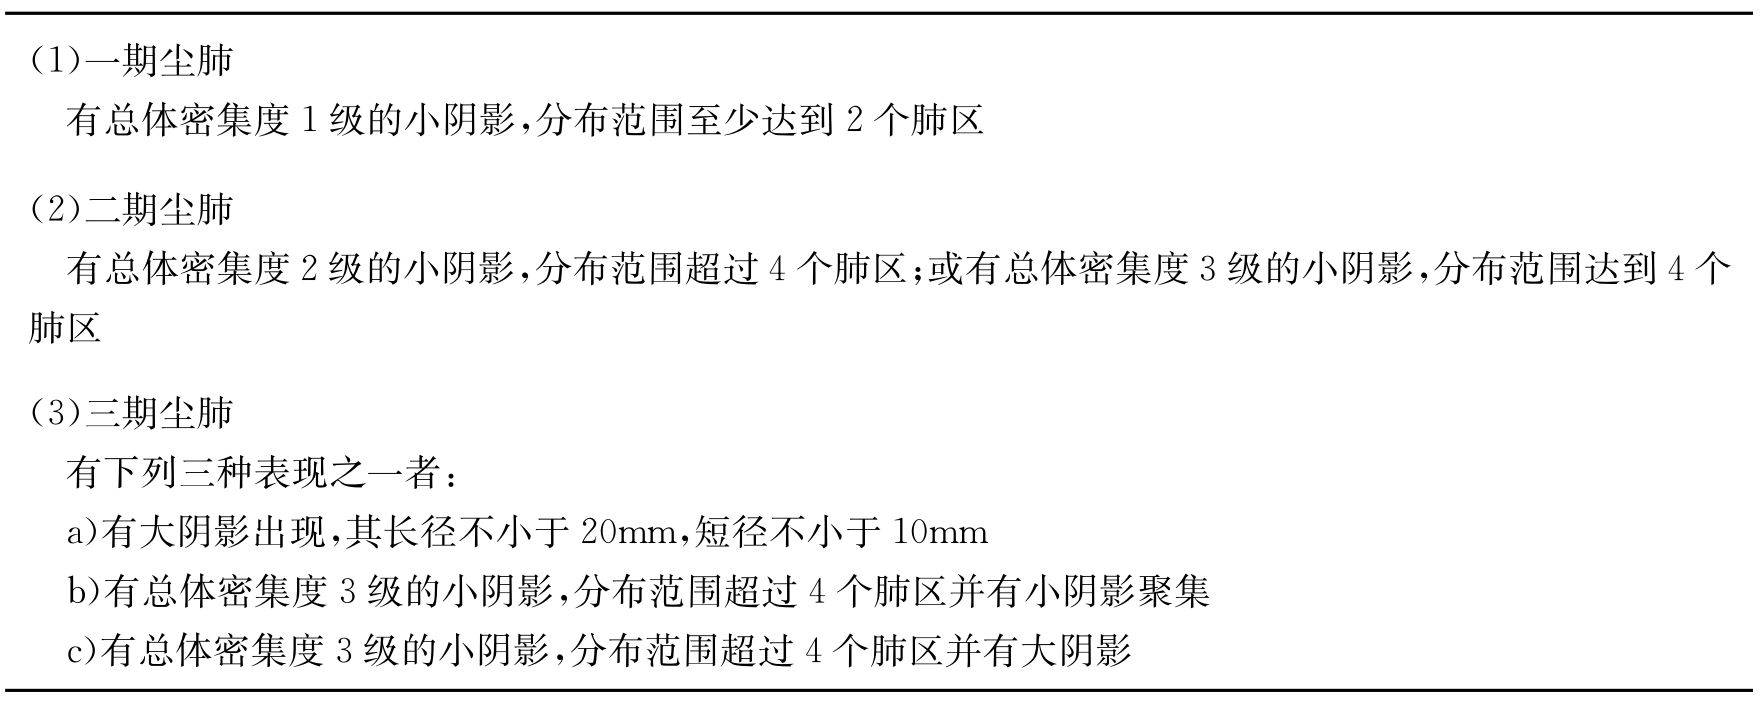
\includegraphics[width=5.86458in,height=2.34375in]{./images/Image00047.jpg}
\end{table}

\paragraph{[附] 硅沉着病并发肺结核}

硅沉着病并发肺结核(硅沉着病结核)是指各期硅沉着病合并肺结核,发生率可高达20\%~90\%。其特点是肺结核的发生率和严重程度常与硅沉着病的发展程度成正比,硅沉着病愈严重,其并发肺结核的可能性愈大,肺结核病病变也较严重,一~二期硅沉着病约10\%~30\%并发肺结核,三期硅沉着病可高达50\%~90\%,是影响预后的主要因素之一。

硅沉着病患者合并肺结核时,肺结核病变往往发展迅速,病灶易溶解为空洞,空洞常巨大而多个。如硅沉着病患者咳嗽咳痰加重、消瘦、气促以及中毒症状进行性加剧,尤其出现潮热、盗汗、咯血、血沉加速、肺上部出现湿啰音而无其他原因可解释者,常提示并发肺结核的可能。痰结核菌阳性对诊断有决定性意义。但硅沉着病合并肺结核时,痰结核菌不一定能在早期找到,因此痰菌阴性不能排除硅沉着病合并肺结核。在胸部X线照片上,肺结核病灶常出现于上肺,形状为多样性,分布不匀,有时成大片阴影,其中可见到空洞,其他肺野内也可有不规则的浸润病灶。

硅沉着病并发浸润性肺结核的X线征有时与三期硅沉着病类似,须加以鉴别,主要有如下几点:①结核病灶一般分布不均匀、左右不对称,病变常单侧性,多形性,而硅结节融合病灶多为两肺对称,呈所谓翼状(或八字状)阴影;②结核病灶形状不规则,活动性病灶呈片状边缘模糊阴影,进展快,并常有空洞形成,病灶与肺门间常有索状阴影相连,病变形态改变快,而硅结节融合病灶常呈圆形或长圆形,边缘较清楚,进展慢,少有空洞形成;③抗结核治疗后,结核病灶可有好转,而硅沉着病结节则无改变。

\subsubsection{(二)矽酸盐肺}

矽酸盐肺是由于长期吸入石英化合物的粉尘所致的尘肺,以石棉肺为最常见。滑石肺、水泥尘肺也属此类。

\paragraph{1.石棉肺}

长期吸入石棉粉尘可引起石棉肺,病情发展缓慢,发病须经7~9年或更长时间。空气中的石棉尘埃浓度愈低,则发病时间愈慢。常见症状有咳嗽、气短与胸痛。胸痛在吸气时较明显,但不经常出现,也无固定部位。痰中可发现石棉小体。此病的X线征象为肺中、下肺野呈网状纤维化阴影,杂有约1mm大小的颗粒状阴影,并有不同程度的肺气肿和胸膜增厚粘连。根据患者的职业史及X线表现,石棉肺不难与硅沉着病鉴别,两者的粉尘接触史不同,石棉肺的X线征象以双下肺网状、条索状阴影为主,而结节的成分很少。石棉肺合并肺结核比较少见,如并发肺结核也不如硅沉着病的严重。石棉肺并发肺癌者却较多。

\paragraph{2.滑石肺}

单纯滑石粉尘的致病力较低,发病的时间较慢,一般发病在10年以上,大多数患者无明显症状。其肺部X线征象为弥散性网状纤维性变及少数边缘不清的斑点状阴影,主要分布于中、下肺野。可根据其粉尘接触史的不同,X线呈网状纤维性变为主而与硅沉着病相鉴别。

滑石肺可见于橡胶、陶瓷、化妆品等工业及滑石采矿工人。由于采用原料的成分中含有不同程度的二氧化矽,因而肺部的病理改变随之而不同,可呈混合性尘肺改变。

\paragraph{3.水泥尘肺}

水泥尘肺发生较迟、发展较慢,主要临床表现为慢性咳嗽、咳痰。后期有肺功能不全的表现。吸入水泥原料粉尘尤以水泥磨石车间及大窑工人比较容易致病,而成品的粉尘不易致病。X线征以网状纤维性变为主,以及散在性、密度不高、边缘不清、分布不一的小结节,后期伴有不同程度的肺气肿。

\subsubsection{(三)煤肺}

煤肺乃由于长期吸入煤尘所致,其发病年龄和工龄较晚,工龄在20年左右,进展也较缓慢,主要症状有慢性咳嗽,咳黑色痰,胸痛及气短等。咳嗽、咳痰较硅沉着病明显,呼吸功能损害较少。主要X线征象是双肺网状纤维阴影,杂有致密度较低的斑点状阴影,斑点大小约1~2mm,上述改变以中、下肺为主,后期也可出现大块状阴影。

煤肺与硅沉着病的区别根据其职业史、症状轻以及X线改变的不同而不难区别。

煤矿工人中的掘进工,其罹患的尘肺基本上属于硅沉着病一类,而井下工人(采煤工,装、运煤工)的尘肺则属于煤肺一类;另有既在岩层又在煤层工作者,可产生以煤肺为主或以硅沉着病为主的混合尘肺。

\subsubsection{(四)肺铁末沉着症}

肺铁末沉着症患者一般无症状,或有不定时的气闷感、咳嗽、胸痛。X线表现为双侧中、下肺纹理增强和斑点状、从针头大至3mm大、边缘清楚、从来不融合成块状阴影,此与硅沉着病不同。肺门阴影不如硅沉着病或石棉肺的大。铁末沉着症很少并发肺结核或其他肺部炎症,劳动能力少有明显损害。其与硅沉着病的鉴别,除参考上述不同的X线征外,粉尘接触史的不同尤其重要(参见第29节)。

\subsubsection{(五)肺锡末沉着症}

吸入氧化锡末可引起肺锡末沉着症,患者一般无明显症状,或有轻咳,个别患者可听到呼吸音粗糙及间断的干啰音(参见第29节)。

\protect\hypertarget{text00066.html}{}{}

\section{16 系统性疾病}

\subsection{一、肺肉芽肿性多血管炎}

亦称Wegener肉芽肿(WG),是一种系统性、坏死性肉芽肿性血管炎,其中70\%~80\%有肺损害。70\%以上患者上呼吸道最先受累,如鼻塞、鼻窦部疼痛、脓性或血性分泌物。鼻咽部溃疡、鼻咽部骨与软骨破坏致鼻中隔或软腭穿孔。肺部病变常引起咳嗽、咯血、胸痛和呼吸困难。多数患者在病程中有不同程度的肾小球肾炎,有血尿、蛋白尿、管型等。X线肺部检查,可见双侧性或单侧性、单发性或多发性结节状或固定浸润阴影,可有厚壁或薄壁空洞形成。也可出现眼部病变、皮肤损害与皮下结节形成等。如病变仅累及肺脏,须与肺结核、非特异性炎症、结节病、肺恶性肿瘤等相鉴别;有空洞形成时又须与肺脓肿相鉴别。实验室指标如c-ANCA(胞浆型抗中性粒细胞胞浆抗体)阳性有较大的诊断价值。诊断参见第5.3节。

\subsection{二、其他风湿性疾病}

系统性红斑狼疮可有间质性肺炎等肺部表现,常与胸膜炎并发。狼疮性肺炎多有白细胞减少,且抗生素治疗无效,激素治疗后肺炎迅速消退。硬皮病、结节性多动脉炎、干燥综合征等也可有肺部病变伴相应的症状。结缔组织病所致肺部病变,须与各种原因所致肺部病变相鉴别,尤以肺部感染。

\subsection{三、尿毒症肺}

尿毒症肺又称尿毒性肺水肿、尿毒性肺炎,是慢性肾衰竭发展到尿毒症期常见的肺部并发症。尿毒症肺X线胸片可呈“蝴蝶状”或“蝙蝠翼状”改变。尿毒症肺发病率在尿毒症患者中高达60\%以上。主要临床表现为轻、中度咳嗽、咳痰及呼吸困难,可有中、小量咯血。肺部听诊可有湿啰音,少数有干啰音。近半数患者可并发胸腔积液。

\subsection{四、热带嗜酸性粒细胞增多症}

热带嗜酸性粒细胞增多症是热带与亚热带地区较常见的疾病,在我国华南与华东地区较为多见,而新疆、东北、内蒙古自治区等地也有发现。临床特点为长期阵发性咳嗽或哮喘并伴有嗜酸性粒细胞增多。

目前普遍认为本病的发病和丝虫感染有关,其中抗体机制和嗜酸性粒细胞在发病机制中可能起重要作用。患者以20~40岁的青壮年为多,女性多于男性。病程多数在3~8个月之间,最短约为1个月,最长可达20年。

起病一般徐缓,以疲乏、食欲减退、体重减轻、微热、咳嗽等为早期症状,咳嗽逐渐加剧,夜间较重且多为阵发性。常伴有肺部哮鸣音与呼气性呼吸困难。痰量不多,呈白色泡沫样,偶可带血。部分病例有胸部不适或压迫感。体检可在过半数病例中听到干啰音,约1/4~1/3病例有湿啰音。约半数病例有浅表淋巴结(颈淋巴结较显著)肿大与轻度肝、脾大。外周血白细胞总数增高,通常>10.0×10\textsuperscript{9}
/L,偶尔可达(40~50)×10\textsuperscript{9}
/L,分类计数嗜酸性粒细胞常在20\%以上,可高达90\%,绝对值>2.0×10\textsuperscript{9}
/L。抗丝虫抗原的补体结合抗体效价增高,血冷凝集试验滴度增高,半数病例可有康氏反应呈暂时性阳性,γ球蛋白增高。支气管肺泡灌洗液中细胞总数及分类计数中嗜酸性粒细胞百分比均明显增高。X线胸片轻者可无异常,典型者有双肺弥漫性分布均匀一致边界不清的小片状、小结节和斑点模糊阴影,直径2~5mm,部分可互相融合而酷似肺炎改变。病变多位于双侧中下肺野,部分可见胸腔积液或空洞形成。慢性者形成肺间质纤维化。

典型病例的诊断主要根据:①长期阵发性咳嗽或哮喘,多半于夜间发作或加剧;②嗜酸性粒细胞计数绝对值增多,致白细胞总数增多;③X线胸片上双肺弥漫性分布均匀一致边界不清的小片状、小结节和斑点模糊阴影;④乙胺嗪或胂剂治疗常有良效。

本病的病程经过可分为急性型、慢性型(经过一年以上)及逍遥型三种类型。逍遥型的诊断较为困难,患者常无特别的主诉,或仅自觉软弱乏力,无长期的咳嗽与气喘史,肺部检查可完全正常,诊断主要根据血象检查,并排除其他原因所致的嗜酸性粒细胞增多症,最后经诊断性治疗的疗效证实诊断。

本病与支气管哮喘的鉴别要点为:①患者家族与自身过去无哮喘病史;②气候转变与哮喘发作无重大关系;③白细胞总数增多,分类嗜酸性粒细胞常在20\%以上(此种情况一般不见于支气管哮喘);④病情经过迁延,症状缓解不完全,而支气管哮喘在间歇期全无症状;⑤应用抗过敏药物与支气管舒张药治疗疗效不显著,而胂剂疗效常常显著。

本病与单纯性肺嗜酸性粒细胞增多症(吕弗勒综合征)的鉴别可参考表\ref{tab5-5}。

\begin{table}[htbp]
\centering
\caption{热带嗜酸性粒细胞增多症与吕弗勒综合征的鉴别诊断}
\label{tab5-5}
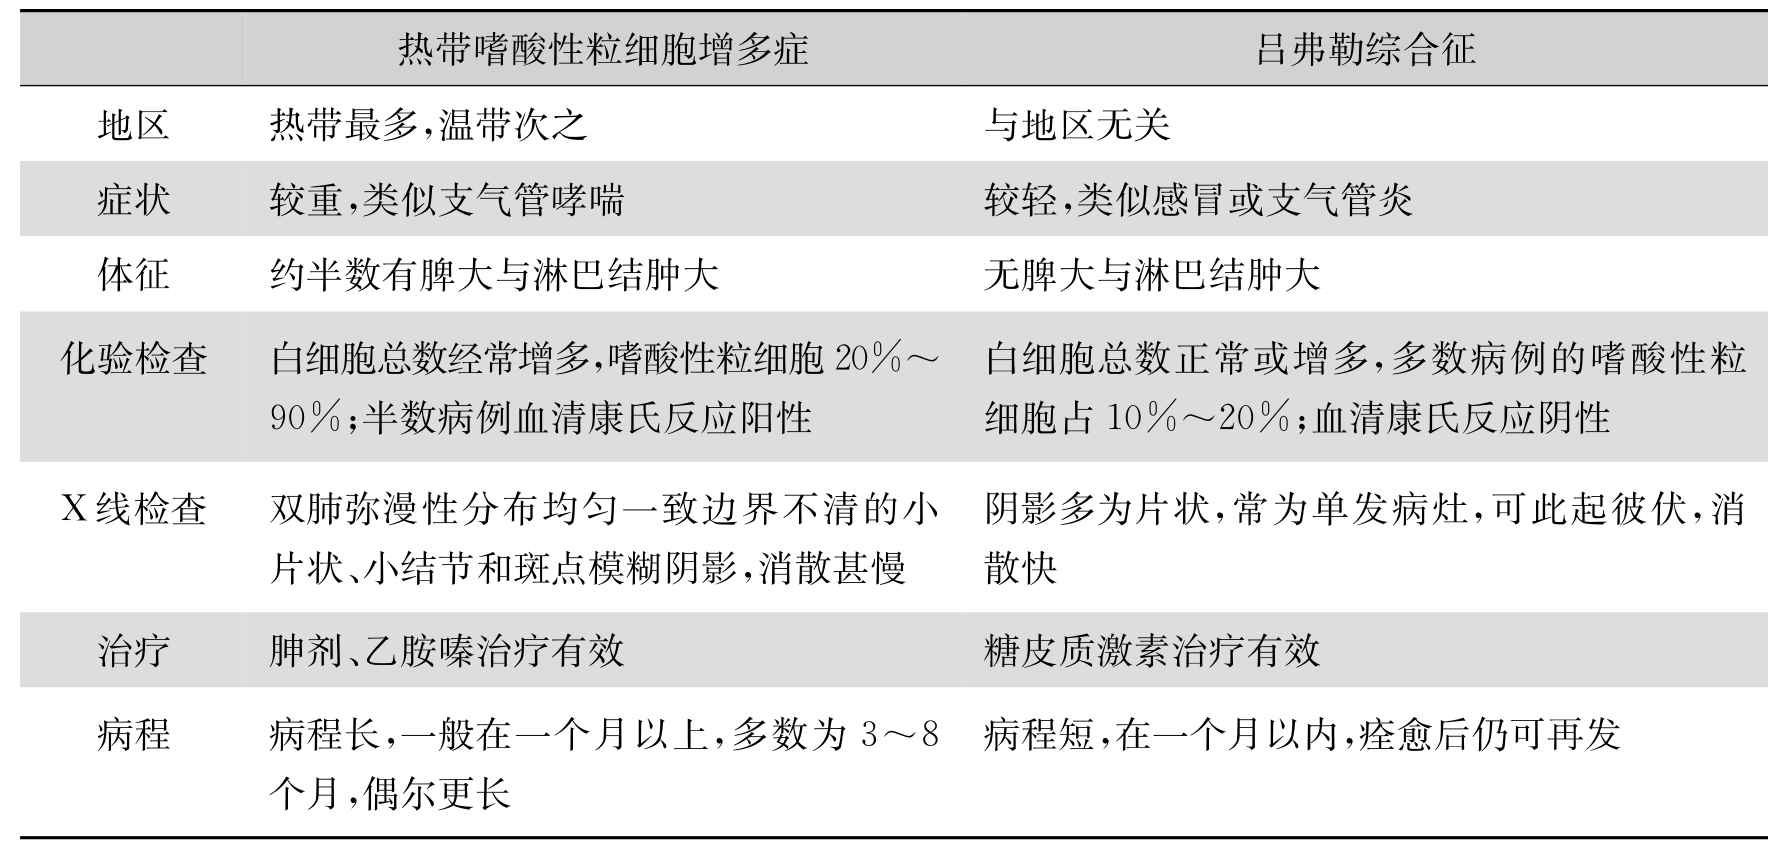
\includegraphics[width=5.91667in,height=2.82292in]{./images/Image00048.jpg}
\end{table}

\protect\hypertarget{text00067.html}{}{}

\section{17 其他}

\subsection{一、胃食管反流}

胃食管反流(GER)是引起不明原因慢性咳嗽的主要病因之一,慢性咳嗽可以是GER的唯一临床表现,但是GER并不一定都引起咳嗽。GER导致咳嗽的机制可能有:①食管远端可能存在咳嗽感受器,受酸刺激导致远端食管-气管支气管迷走神经反射,引起咳嗽;②近端食管反流物的微量吸入或大量吸入,引起咳嗽。患者的临床表现为慢性咳嗽,部分可伴有反流症状如反酸、胃灼热、胸骨后不适和疼痛、咽炎、口腔溃疡等。24小时食管pH监测是GER的最敏感和特异的检查,不仅可以检测反流发生的持续时间和频率,还可确定咳嗽和反流发作的时间关系,若二者发作的时间关系存在,即使反流参数正常亦可确定反流为咳嗽的病因。

临床上若患者咳嗽时间超过3个月,常规治疗无效,同时伴有胃部症状而胸部X线、肺功能及组胺激发试验、鼻部检查均正常,则要考虑GER性咳嗽的可能,行24小时食管pH监测若反流与咳嗽的症状相关概率(SAP)≥95\%可以做出初步诊断(国内指南以75\%为标准,较国际指南低),如抗反流试验性治疗有效则可以确诊。注意GER性咳嗽药物治疗一般需2~3个月方有症状改善,5~6个月咳嗽方能消失,故试验性治疗不宜短于4周,常用的药物包括H\textsubscript{2}
受体拮抗剂加促胃动力药,或质子泵抑制剂。

诊断标准:①慢性咳嗽,以白天咳嗽为主;②24小时食管pH值监测Demeester积分≥12.70,及(或)SAP≥75\%;③抗反流治疗后咳嗽明显减轻或消失。但抗反流药物对20\%的胃食管反流相关咳嗽无效,治疗失败也不能完全排除,需进一步检查明确。

\subsection{二、药物性咳嗽}

血管紧张素转换酶抑制剂(ACEI)如卡托普利、依那普利、培哚普利、赖诺普利等可诱发咳嗽,主要表现为慢性持续性干咳,伴喉部刺激感,夜间及卧位加重,可在首次服药数小时内出现,也可以在数周或数月内出现,与剂量大小无关。国外资料显示大约10\%~30\%的慢性咳嗽是由于使用ACEI引起的,其发生机制尚未十分明确,但目前倾向于ACEI抑制了缓激肽的代谢,以及P物质、组织胺、前列腺素等炎症介质增加,刺激咳嗽感受器产生咳嗽;另外可能与遗传基因有关。任何服用ACEI类药物患者发生咳嗽时均应考虑本诊断,但须排除其他病因所致咳嗽。无论咳嗽在服用ACEI类药物多久后出现,均可停用ACEI以确定诊断,ACEI相关性咳嗽将于停药4周后消失或减轻。

胺碘酮也能引起持续性干咳。

\subsection{三、腹膜透析}

腹膜透析患者比血液透析患者更易发生咳嗽,虽然两者均接受药物治疗,如ACEI、β受体阻滞剂等可诱发咳嗽,腹透和血透也可由于液体负荷过大及肺水肿产生咳嗽。目前认为腹透主要由于胃食管反流所致,故对腹透患者如有咳嗽应对上述危险因素进行排查。

\subsection{四、阿诺尔德神经反射性咳嗽综合征}

正常人外耳道存在咳嗽感受器,异物(毛发、耵聍)等机械刺激可通过阿诺尔德(Arnold)神经(迷走神经耳支)传入咳嗽中枢引起咳嗽。外耳或中耳疾病有时可压迫阿诺尔德神经,引起难治性咳嗽。解除病因后咳嗽症状可消失。

\subsection{五、精神性咳嗽}

也称心因性咳嗽,发生率较低,多见于儿童和青少年,其特点为干咳,声音特别响亮,有人在旁时咳嗽加剧,分散注意力或睡眠时消失,止咳治疗无效。成人精神性咳嗽则可在睡眠时发生,咳嗽持续时间更长。凡经各种检查排除各种器质性疾患者可确定诊断。治疗应采取心理治疗,常需治疗数周至数月才能见效。

\subsection{六、不明原因慢性咳嗽}

临床上有一部分慢性咳嗽患者在经过全面检查后病因未能明确,称为不明原因慢性咳嗽或慢性特发性咳嗽。通常指临床上咳嗽作为呼吸系统表现的唯一症状,持续时间超过8周,胸部影像学未见异常,未使用血管紧张素转换酶抑制剂(ACEI)者。在国外不明原因的慢性咳嗽患者约占呼吸门诊的14\%~23\%。国内报道一组86例不明原因的慢性咳嗽患者中最常见的病因依次是咳嗽变异型哮喘(27.9\%)、鼻后滴流综合征(25.6\%)、嗜酸性粒细胞性支气管炎(15.1\%)、胃食管反流(14.0\%),它们单独或者合并引起不明原因慢性咳嗽病因的约89.5\%。因此,不明原因慢性咳嗽如经细致的检查大多可明确病因。

\subsection{七、咳嗽高敏感综合征}

近年来提出咳嗽高敏感综合征(cough hypersensitivity
syndrome,CHS)来描述慢性咳嗽患者,其定义主要指咳嗽敏感性升高、全面检查及治疗后仍未能明确病因的慢性咳嗽患者。临床特征主要表现为慢性刺激性干咳,对一种或多种咳嗽激发物如冷空气、讲话及气味等敏感,咽喉部存在咳嗽冲动,并且严重影响患者生活质量。患者以中年女性较多,经常以上呼吸道感染作为起病的首发因素。

\protect\hypertarget{text00068.html}{}{}

\section{参考文献}

1.蔡柏蔷.慢性肾衰的肺部并发症.中华结核和呼吸杂志,1997,20(1):9

2.马洪明,等.不明原因慢性咳嗽的诊断探讨.中华结核和呼吸杂志,2003,26(11):675

3.赖克方,等.加强不明原因慢性咳嗽的病因诊断研究.中华内科杂志,2003,42(7):451

4.马洪明,等.嗜酸粒细胞性支气管炎的气道炎症和临床特点.中华结核和呼吸杂志,2003,26(6):362

5.张永祥,等.嗜酸粒细胞性支气管炎九例临床分析.中华内科杂志,2002,41(7):480

6.于润江.注意识别弥漫性泛细支气管炎.中华内科杂志,2000,39(1):8

7.刘少滨,等.弥漫性泛细支气管炎一例.中华结核和呼吸杂志,2000,23(3):157

8.李英姬,等.弥漫性泛细支气管炎和大环内酯类药物疗法.中华结核和呼吸杂志,2002,25(7):421

9.辛建保,等.慢性干咳伴有气道高反应性即是咳嗽变异性哮喘吗?中华结核和呼吸杂志,1998,21(3):138

10.王巍,等.支气管结核诊断治疗近况.中华结核和呼吸杂志,2000,23(5):306

11.林金学,等.单纯气管、支气管结核病28例临床分析.中华结核和呼吸杂志,1997,20(6):368

12.张平,等.纤维素性支气管炎二例.中华结核和呼吸杂志,2002,25(2):101

13.谢伶华.弥漫性肺泡癌误诊为粟粒性肺结核13例.中华结核和呼吸杂志,2000,23(4):251

14.曹彬,等.肺隐球菌病临床分析.中华结核和呼吸杂志,2002,25(10):610

15.褚海青,等.肺隐球菌病19例临床分析.中华内科杂志,2003,42(9):650

16.易祥华,等.10例肺隐球菌病病理和影像学对照分析.中华结核和呼吸杂志,2000,23(9):574

17.李瑞慧,等.肺奴卡菌病二例.中华传染病杂志,2001,19(3):136

18.刁晓源,等.肺放线菌病二例.中华结核和呼吸杂志,1995,18(4):238

19.谢灿茂,等.人类比翼线虫病三例.中华内科杂志,1998,37(5):345

20.杨光钊,等.肺泡蛋白沉积症的高分辨率CT表现.中华放射学杂志,2002,36(5):467

21.张孔,等.韦格纳肉芽肿病肺损害的临床分析.中华结核和呼吸杂志,2003,26(10):623

22.郭强,等.系统性红斑狼疮患者525例肺部病变的调查.中华风湿病学杂志,2004,8(6):363

23.朱礼星,等.胃食管反流性咳嗽的临床分析.中华内科杂志,2003,42(7):461

24.李兆申,等.胃食管反流病诊疗现状及面临的问题.中华内科杂志,2004,43(7):548

25.马洪明,等.嗜酸性粒细胞性支气管炎的气道炎症和临床特点.中华结核和呼吸杂志,2003,26(6):362

26.于润江.注意识别弥漫性泛细支气管炎.中华内科杂志,2000,39(1):8

27.刘少滨,等.弥漫性泛细支气管炎一例.中华结核和呼吸杂志,2000,23(3):157

28.李英姬,等.弥漫性泛细支气管炎和大环内酯类药物疗法.中华结核和呼吸杂志,2002,25(7):421

29.张平,等.纤维素性支气管炎二例.中华结核和呼吸杂志,2002,25(2):101

30.谢伶华.弥漫性肺泡癌误诊为粟粒性肺结核13例.中华结核和呼吸杂志,2000,23(4):251

31.曹彬,等.肺隐球菌病临床分析.中华结核和呼吸杂志,2002,25(10):610

32.褚海青,等.肺隐球菌病19例临床分析.中华内科杂志,2003,42(9):650

33.易祥华,等.10例肺隐球菌病病理和影像学对照分析.中华结核和呼吸杂志,2000,23(9):574

34.李瑞慧,等.肺奴卡菌病二例.中华传染病杂志,2001,19(3):136

35.杨光钊,等.肺泡蛋白沉积症的高分辨率CT表现.中华放射学杂志,2002,36(5):467

36.张孔,等.韦格纳肉芽肿病肺损害的临床分析.中华结核和呼吸杂志,2003,26(10):623

37.郭强,等.系统性红斑狼疮患者525例肺部病变的调查.中华风湿病学杂志,2004,8(6):363

38.朱礼星,等.胃食管反流性咳嗽的临床分析.中华内科杂志,2003,42(7):461

39.李兆申,等.胃食管反流病诊疗现状及面临的问题.中华内科杂志,2004,43(7):548

40.中华医学会呼吸病学分会哮喘学组.咳嗽的诊断与治疗指南(2009版).中华结核和呼吸杂志,2009,32
(6):407-413.

41.中华医学会结核病学分会.气管支气管结核诊断和治疗指南(试行).中华结核和呼吸杂志,2012,35(8).

42.Jaklitsch MT,et al.The American Association for Thoracic Surgery
guidelines for lung cancer screening using low-dose computed tomography
scans for lung cancer survivors and other high-risk groups.J Thorac
Cardiovasc Surg.2012;144:33-38.

43.Morice AH.Chronic cough hypersensitivity syndrome.Cough.2013,9:14.

44.Tarlo SM.Peritoneal dialysis and cough:ACCP evidence-based clinical
practice guidelines.Chest.2006;129 (1Suppl):202S-203S

45.Brown KK.Chronic cough due to chronic interstitial pulmonary
diseases:ACCP evidence-based clinical practice
guidelines.Chest.2006;129(1Suppl):180S-185S

46.Vijayan VK.Tropical pulmonary eosinophilia:pathogenesis,diagnosis
and management.Curr Opin Pulm Med.2007;13:428-433.

\protect\hypertarget{text00069.html}{}{}

